% ============================================================
% MTH321 Project 2 (PDE BVP) — Team F report
% Visual system aligned with Project 1 FINAL (TeamF_Report.tex):
% Palatino/mathpazo, navy accents, crest title page.
% r4 (2026-11-13): Appendices A--B filled; signatures from report/signatures/.
% r5 (2026-11-14): all appendices/ICS filled; placeholder macros disabled; production copy of ai_check/main_r5_cand.tex.
% Compile: /tmp/tectonic -k --keep-logs main.tex  (or pdflatex twice).
% ============================================================
\documentclass[11pt,a4paper]{article}

\usepackage[utf8]{inputenc}
\usepackage[T1]{fontenc}
% ---- type: Palatino text + math (URW Palladio via mathpazo, true small caps), as in P1 FINAL -------------
\usepackage{amsmath, amssymb, amsthm}
\usepackage[sc]{mathpazo}
\linespread{1.05}
\renewcommand{\ttdefault}{txtt}            % monospaced companion with Palatino-like colour (txfonts)
\usepackage{geometry}
\geometry{a4paper, margin=2.5cm, headheight=14pt, headsep=8mm, footskip=12mm}   % template: margin=2.5cm
\usepackage{graphicx}
\usepackage{booktabs}
\usepackage{xcolor}
\usepackage{enumitem}
\usepackage{float}
\usepackage{caption}
\usepackage{subcaption}
\usepackage{bm}
\usepackage{algorithm}
\usepackage{algpseudocode}
\usepackage{mdframed}
\usepackage{array}
\usepackage{iftex}
\ifPDFTeX
  \usepackage[protrusion=true,expansion=true,tracking=true,kerning=true]{microtype}
\else
  % tectonic/XeTeX: expansion unsupported; keep protrusion/tracking/kerning
  \usepackage[protrusion=true,expansion=false,tracking=true,kerning=true]{microtype}
\fi
\usepackage[section]{placeins}
\usepackage{titlesec}
\usepackage{needspace}
\usepackage{tabularx}
\usepackage{ragged2e}
\usepackage{fancyhdr}
\setlength{\emergencystretch}{1.5em}
\usepackage{hyperref}
\usepackage{xurl}
\urlstyle{same}
\widowpenalty=10000 \clubpenalty=10000 \displaywidowpenalty=10000

% ---- palette (identical to P1 / the slides) ---------------------------------------------------------------------
\definecolor{ink}{HTML}{1F2933}
\definecolor{accent}{HTML}{23426B}
\definecolor{muted}{HTML}{4B5563}
\definecolor{note}{HTML}{374151}
\definecolor{hairline}{HTML}{C9CDD2}
\definecolor{formbg}{RGB}{250,250,245}       % course template colours (kept defined)
\definecolor{formframe}{RGB}{180,170,140}
\definecolor{todo}{RGB}{156,74,60}
\AtBeginDocument{\color{ink}}

% --- r5: all placeholders filled; placeholder macros disabled so any leftover use fails to compile ---
% \newcommand{\PH}[1]{\colorbox{yellow}{\textsf{\footnotesize[TO FILL: #1]}}}
% \newcommand{\PHc}{\colorbox{yellow}{\textsf{\footnotesize[TO FILL]}}}
\newmdenv[backgroundcolor=formbg,linecolor=formframe,linewidth=0.8pt,roundcorner=3pt,
  innermargin=5pt,outermargin=5pt,innertopmargin=8pt,innerbottommargin=8pt]{formbox}
% \newmdenv[backgroundcolor=yellow!60,linecolor=orange,linewidth=0.8pt,innertopmargin=6pt,innerbottommargin=6pt]{phbox}

\hypersetup{colorlinks=true,linkcolor=accent,citecolor=accent,urlcolor=accent,
  pdftitle={Mixed Boundary Data for the Poisson Equation},pdfauthor={Team F},
  pdfsubject={MTH321 Project 2 (Direction 2: Elliptic BVP with Mixed Boundary Conditions) Report}}
\graphicspath{{figures/}}

% ---- headings: navy numbers, small-caps subsections, one hairline under sections ---------------------------
\titleformat{\section}[block]{\normalfont\Large\color{ink}}{\color{accent}\thesection}{0.9em}{}
  [\vspace{1.2ex}{\color{hairline}\titlerule[0.4pt]}]
\titlespacing*{\section}{0pt}{3.0ex plus 1ex minus .2ex}{2.0ex plus .3ex}
\titleformat{\subsection}{\normalfont\large\scshape\color{ink}}{\color{accent}\thesubsection}{0.9em}{}
\titlespacing*{\subsection}{0pt}{14pt plus 4pt minus 2pt}{6pt plus 1pt}
\titleformat{\subsubsection}{\normalfont\itshape}{\thesubsubsection}{0.8em}{}
\titleformat{\paragraph}[runin]{\normalfont\itshape\color{ink}}{}{0pt}{}[\upshape\hspace{0.15em}]
\titlespacing*{\paragraph}{0pt}{1.4ex plus .5ex minus .2ex}{0.6em}
\newcommand{\sectionbreak}{\Needspace{8\baselineskip}}
\newcommand{\subsectionbreak}{\Needspace{7\baselineskip}}
\newcommand{\lead}[1]{{\scshape\color{accent}#1}}   % small-caps run-in label
\newcommand{\runin}[1]{\textit{#1}}                 % run-in labels in the body: italic, not bold

% ---- table of contents ----------------------------------------------------------------------------------------
\makeatletter
\renewcommand{\l@section}[2]{\addpenalty{-\@highpenalty}\vskip 0.55em plus 1pt
  {\parindent\z@\rightskip\@pnumwidth\parfillskip -\@pnumwidth
   \leavevmode\normalsize\@tempdima 1.6em\advance\leftskip\@tempdima\hskip -\leftskip
   {\color{ink}#1}\nobreak\hfil\nobreak\hb@xt@\@pnumwidth{\hss\color{ink}#2}\par}}
\renewcommand{\@dotsep}{1000}                      % no leader dots
\makeatother

% ---- running heads -------------------------------------------------------------------------------------------
\pagestyle{fancy}
\fancyhf{}
\renewcommand{\headrulewidth}{0pt}
\fancyhead[L]{\footnotesize\color{muted}\textsc{mixed boundary data}\ \textperiodcentered\ \textsc{team f}}
\fancyhead[R]{\footnotesize\color{muted}\itshape\nouppercase{\rightmark}}
\fancyfoot[C]{\small\color{muted}\thepage}
\renewcommand{\sectionmark}[1]{\markboth{\thesection\quad #1}{\thesection\quad #1}}
\renewcommand{\subsectionmark}[1]{}
\fancypagestyle{plain}{\fancyhf{}\renewcommand{\headrulewidth}{0pt}\fancyfoot[C]{\small\color{muted}\thepage}}

% ---- captions, tables, lists ---------------------------------------------------------------------------------
\DeclareCaptionFont{accent}{\color{accent}}
\DeclareCaptionFont{note}{\color{note}}
\DeclareCaptionFont{ink}{\color{ink}}
\captionsetup{font=small,labelfont={sc,accent},textfont={normalfont,ink},labelsep=period,
  justification=raggedright,singlelinecheck=false,margin=0pt}
\captionsetup[table]{skip=6pt,position=top}
\captionsetup[figure]{skip=6pt}
\captionsetup[algorithm]{font=small,labelfont={sc,accent},textfont={normalfont,ink},format=hang}
\setlength{\heavyrulewidth}{0.6pt}\setlength{\lightrulewidth}{0.35pt}\setlength{\cmidrulewidth}{0.35pt}
\setlength{\aboverulesep}{0.4ex}\setlength{\belowrulesep}{0.6ex}
\renewcommand{\arraystretch}{1.12}
\newcommand{\apptabfont}{\small}
\setlist{itemsep=2pt,topsep=4pt}
\setlist[itemize]{label={\color{muted}\textendash}}
\setlength{\textfloatsep}{12pt plus 2pt minus 2pt}
\setlength{\floatsep}{12pt plus 3pt minus 3pt}
\setlength{\intextsep}{9pt plus 2pt minus 2pt}
\renewcommand{\topfraction}{0.85}\renewcommand{\bottomfraction}{0.6}\renewcommand{\textfraction}{0.12}
\renewcommand{\floatpagefraction}{0.75}\setcounter{topnumber}{3}\setcounter{totalnumber}{4}

% ---- theorem-like environments (same names/numbering as previous P2; small-caps navy labels) -------------
\newtheoremstyle{palplain}{1.2ex plus .4ex}{1.2ex plus .4ex}{\itshape}{0pt}{\scshape\color{accent}}{.}{0.5em}
  {\thmname{#1}\thmnumber{ #2}\thmnote{ {\normalfont\color{muted}(#3)}}}
\newtheoremstyle{paldef}{1.2ex plus .4ex}{1.2ex plus .4ex}{\normalfont}{0pt}{\scshape\color{accent}}{.}{0.5em}
  {\thmname{#1}\thmnumber{ #2}\thmnote{ {\normalfont\color{muted}(#3)}}}
\newtheoremstyle{palremark}{1.0ex plus .4ex}{1.0ex plus .4ex}{\normalfont}{0pt}{\itshape}{.}{0.5em}{}
\theoremstyle{palplain}
\newtheorem{theorem}{Theorem}[section]
\newtheorem{lemma}[theorem]{Lemma}
\newtheorem{proposition}[theorem]{Proposition}
\newtheorem{corollary}[theorem]{Corollary}
\theoremstyle{paldef}
\newtheorem{definition}[theorem]{Definition}
\newtheorem{assumption}[theorem]{Assumption}
\theoremstyle{palremark}
\newtheorem{remark}[theorem]{Remark}

% ---- algorithm style ---------------------------------------------------------------------------------------
\algrenewcommand{\algorithmicrequire}{\textsc{Input:}}
\algrenewcommand{\algorithmicensure}{\textsc{Output:}}
\algrenewcommand{\algorithmicend}{\textsc{end}}\algrenewcommand{\algorithmicdo}{\textsc{do}}
\algrenewcommand{\algorithmicwhile}{\textsc{while}}\algrenewcommand{\algorithmicfor}{\textsc{for}}
\algrenewcommand{\algorithmicforall}{\textsc{for all}}\algrenewcommand{\algorithmicloop}{\textsc{loop}}
\algrenewcommand{\algorithmicrepeat}{\textsc{repeat}}\algrenewcommand{\algorithmicuntil}{\textsc{until}}
\algrenewcommand{\algorithmicprocedure}{\textsc{procedure}}\algrenewcommand{\algorithmicfunction}{\textsc{function}}
\algrenewcommand{\algorithmicif}{\textsc{if}}\algrenewcommand{\algorithmicthen}{\textsc{then}}
\algrenewcommand{\algorithmicelse}{\textsc{else}}\algrenewcommand{\algorithmicreturn}{\textsc{return}}
\algrenewcommand{\algorithmiccomment}[1]{\hfill\textcolor{muted}{\# #1}}
\makeatletter   % algorithm float: booktabs-weight rules instead of the default 0.8pt rules
\renewcommand\fs@ruled{\def\@fs@cfont{\small\scshape\color{accent}}\let\@fs@capt\floatc@ruled
  \def\@fs@pre{\hrule height\heavyrulewidth depth0pt \kern3pt}%
  \def\@fs@post{\kern3pt\hrule height\lightrulewidth\relax}%
  \def\@fs@mid{\kern3pt\hrule height\lightrulewidth\kern3pt}%
  \let\@fs@iftopcapt\iftrue}
\makeatother

\newcommand{\GD}{\Gamma_D}
\newcommand{\GB}{\Gamma_B}
\newcommand{\dd}{\,\mathrm{d}}

% written by make_tables.py from results/cost_accuracy*.csv
\newcommand{\CostSpreadMatched}{14}
\newcommand{\CostWorstRatio}{1.22}
\newcommand{\CostWorstCase}{Neumann, ghost, $N=32$}

\begin{document}
% ---- title page (P1 visual system; P2 roster roles and existing abstract verbatim) ---
\begin{titlepage}
\pdfbookmark[0]{Title page}{titlepage}
\noindent\begin{minipage}[t]{0.8\textwidth}\vspace{0pt}\raggedright
{\color{note}\small\textsc{Project 2 (Direction 2: Elliptic BVP) Report}}
\end{minipage}\hfill
\begin{minipage}[t]{0.15\textwidth}\vspace{0pt}\raggedleft

\includegraphics[height=17mm]{xjtlu_crest}
\end{minipage}

\vspace{6mm}
\noindent\begin{minipage}{\textwidth}\raggedright
{\color{accent}\fontsize{19}{24}\selectfont Mixed Boundary Data for the Poisson Equation:\par}
\vspace{3.5mm}
{\large\itshape First-Order versus Ghost-Point Closures of a Neumann/Robin Edge\par}
\vspace{7mm}
{\color{hairline}\rule{0.42\textwidth}{0.4pt}}\par
\vspace{6mm}
{\large\scshape Team F}\par
\vspace{2.5mm}
{\renewcommand{\arraystretch}{1.18}%
\begin{tabular}{@{}l@{\hspace{2.2em}}l@{\hspace{2.2em}}>{\itshape\color{note}}l@{}}
Kunze Li & 2363973 & Project Manager\\
Zekun Wang & 2363718 & Visualization \& Report\\
Yawen Wu & 2360749 & Mathematical Theory\\
Che Li & 2362072 & Algorithm Implementation\\
Yixuan Liu & 2361140 & Testing \& Validation\\
Ruitong Huang & 2360294 & Video \& Presentation\\
\end{tabular}}\par
\end{minipage}

\vspace{9mm}
\noindent\begin{minipage}{\textwidth}
{\scshape\color{accent}Abstract}\par\vspace{1.2mm}
\small\setlength{\parindent}{0pt}

We solve the Poisson equation on the unit square with Dirichlet data on three edges,
including all four corners, and Neumann or Robin data on $x=1$, using the five-point stencil.
Two closures of the flux edge are compared on identical grids, data and norms: a one-sided
derivative row that replaces the partial differential equation (PDE) at $x=1$, and a
ghost-point elimination that keeps a PDE row there. Both closures have an $O(h)$ boundary
truncation error, yet their global orders differ: we prove that both matrices are nonsingular
M-matrices and, with discrete comparison functions, derive maximum-norm bounds of order $h$ for
the one-sided row and $h^2$ for the ghost closure. A diagonal scaling of the boundary rows makes
$DA$ symmetric positive definite, so conjugate gradients can be applied to $DAU=DF$. On $u^*=e^{x+y}$ with $N\le256$ the
observed orders are $1$ and $2$ in $L^2_h$ and nodal $L^\infty$, and the measured truncation
constants match the Taylor predictions. A tolerance sweep separates algebraic from
discretisation error, and $\kappa_2(DA)$ grows like $N^2$. At the target
$\|e\|_\infty\le5\times10^{-3}$ the ghost closure needs $N=16$ and the first-order closure
$N=128$ or $256$, a solve-time gap of two to three orders of magnitude. With incompatible data
at the mixed corner, $u^*=\mathrm{Im}(z\,\mathrm{Log}\,z)$, the ghost closure falls to order $1$
in $L^\infty$ near that corner but remains second order away from it on the tested meshes.

\par\vspace{2.2mm}\lead{Keywords:} mixed boundary conditions, Robin condition, ghost point,
truncation error, M-matrix, discrete maximum principle, row scaling.\par
\end{minipage}

\vfill
\noindent{\color{hairline}\rule{\textwidth}{0.4pt}}\par\vspace{2.5mm}
\noindent{\small\color{accent}MTH321 Numerical Analysis of Partial Differential Equations, Xi'an Jiaotong-Liverpool
University\par}\vspace{1mm}
\noindent{\small\color{note}November 2026\par}
\end{titlepage}
\setcounter{page}{2}

{\hypersetup{linkcolor=ink}\tableofcontents}
\newpage


% ============================================================
\section{Introduction and Motivation}
\subsection{Problem Background}
% ============================================================
We study the Poisson problem
\[
-\Delta u=f\quad\text{in }\Omega=(0,1)^2,\qquad
u=g\text{ on }\GD,\qquad
\partial_n u+\beta u=r\text{ on }\GB,
\]
with $\GB=\{1\}\times(0,1)$ and $\GD=\partial\Omega\setminus\GB$, so that all four corners
are treated as Dirichlet nodes. The flux edge is either Neumann ($\beta=0$, $r=q$) or Robin
($\beta=2$). The interior uses the standard five-point stencil; the question is how the
right-edge row is closed. Direction~2 of the Problem Pack compares two closures under identical
settings: a first-order one-sided derivative row that \emph{replaces} the PDE at $x=1$, and a
ghost-point elimination that keeps a PDE row there and builds the boundary condition into the
stencil.

The same mixed pattern is common in applications. Steady heat conduction in a homogeneous
plate yields $-\Delta u=f$ with prescribed temperature on some edges and either a given
heat flux (Neumann) or Newton's law of cooling $\partial_n u+\beta u=r$ (Robin; $\beta$ is the
heat-transfer coefficient divided by the conductivity~\cite{incropera}). In incompressible flow the pressure-Poisson equation obtained from the Navier--Stokes momentum
balance typically carries Neumann data on walls where the normal velocity is prescribed
\cite{gresho}. In both settings the flux edge is part of the model, so the discrete
closure of that edge is part of the method and can set the global accuracy on its own.

Theorem~\ref{thm:conv} turns the truncation defects of rows \eqref{eq:first}--\eqref{eq:ghost}
into maximum-norm error bounds. Tables~\ref{tab:trunc}--\ref{tab:rob} test the predicted
constants and rates, and Table~\ref{tab:cost} compares solve times at a common accuracy target;
Section~\ref{sec:incompat} repeats the comparison with data incompatible at the mixed corner
$(1,0)$, where an exact solution is still available.

\subsection{Research Questions}
\begin{itemize}[leftmargin=2.2em]
  \item[\textbf{Q1.}] Both closures have an $O(h)$ local defect on $\GB$
    (Section~\ref{sec:disc}, Table~\ref{tab:trunc}). Do they still converge at different
    global orders in $L^2_h$ and $L^\infty$, and can these orders be proved for schemes with
    these two boundary rows?
  \item[\textbf{Q2.}] What does each closure do to the linear system (symmetry of $A$, M-matrix
    structure, admissible solvers), and which closure reaches $\|e\|_\infty\le5\times10^{-3}$
    at lower \texttt{spsolve} cost?
  \item[\textbf{Q3.}] When the data are incompatible at the mixed corner, so that the $C^4$
    hypothesis of Theorem~\ref{thm:conv} fails, do the observed orders of the two closures
    drop, and does the maximum error concentrate at that corner?
\end{itemize}

\subsection{Overview of the Report}
Section~\ref{sec:model} states the boundary-value problem (BVP) \eqref{eq:bvp} and its
Lax--Milgram well-posedness. Section~\ref{sec:disc} derives both closures, their truncation
errors, the M-matrix and symmetrisation properties, and the comparison-function bounds of
Theorem~\ref{thm:conv}. Section~\ref{sec:impl} records assembly and the solver choice;
Section~\ref{sec:verif} checks truncation constants, residuals and condition numbers against
the predicted values and separates algebraic from discretisation error with a conjugate
gradient (CG) tolerance sweep; Section~\ref{sec:exp} reports the refinement study, the
cost--accuracy comparison, the incompatible-corner experiment and the limitations;
Section~\ref{sec:concl} answers the Problem Pack question.

% ============================================================
\section{Mathematical Model}\label{sec:model}
% ============================================================
\subsection{Problem statement}
Let $\Omega=(0,1)^2$, $\GB=\{1\}\times(0,1)$ (the open right edge) and
$\GD=\partial\Omega\setminus\GB$ (the edges $x=0$, $y=0$, $y=1$ \emph{including all four
corners}). We seek $u$ with
\begin{equation}\label{eq:bvp}
-\Delta u = f \ \text{in }\Omega,\qquad u=g\ \text{on }\GD,\qquad
\partial_n u+\beta u = r\ \text{on }\GB,
\end{equation}
where $\partial_n u=u_x$ on $\GB$ (outward normal $(1,0)$). The Neumann variant is
$\beta=0$, $r=q$; the Robin variant uses $\beta=2$. For verification we use the
manufactured solution prescribed in the Problem Pack,
\begin{equation}\label{eq:mms}
u^*(x,y)=e^{x+y},\quad f=-2e^{x+y},\quad g=u^*|_{\GD},\quad q(y)=e^{1+y},\quad r(y)=(1+\beta)e^{1+y},
\end{equation}
so $r=3e^{1+y}$ for $\beta=2$. Because $u^*$ increases towards $\GB$, $q=e^{1+y}>0$
confirms the outward-normal sign.

\subsection{Well-posedness}
Let $V=\{v\in H^1(\Omega): v|_{\GD}=0\}$. Multiplying \eqref{eq:bvp} by $v\in V$ and
integrating by parts (Green's formula), with $\partial_n u=r-\beta u$ on $\GB$,
gives the weak problem: find $u\in g_\ast+V$ (with $g_\ast\in H^1(\Omega)$ any lifting of $g$) such that
\begin{equation}\label{eq:weak}
a(u,v):=\int_\Omega\nabla u\cdot\nabla v\dd x+\beta\int_{\GB}uv\dd s
=\int_\Omega fv\dd x+\int_{\GB}rv\dd s=:\ell(v)\qquad\forall v\in V.
\end{equation}

\begin{assumption}\label{ass:data}
$f\in L^2(\Omega)$, $r\in L^2(\GB)$, $g$ is the trace of some $g_\ast\in H^1(\Omega)$, and
$\beta\ge 0$ is constant.
\end{assumption}

\begin{proposition}\label{prop:wellposed}
Under Assumption~\ref{ass:data}, problem \eqref{eq:weak} has a unique solution, and it
depends continuously on $(f,r,g_\ast)$.
\end{proposition}
\begin{proof}
$a$ is bounded on $H^1$ by Cauchy--Schwarz and the trace inequality
$\|v\|_{L^2(\GB)}\le C_T\|v\|_{H^1(\Omega)}$. Because $\GD$ has positive
length, the Friedrichs (Poincaré) inequality $\|v\|_{L^2(\Omega)}\le C_P\|\nabla v\|_{L^2(\Omega)}$
holds on $V$; for $v\in V$ it is elementary here: $v(x,y)=\int_0^y v_y(x,t)\dd t$ gives
$C_P=1/\sqrt2$. Hence, for $\beta\ge 0$,
$a(v,v)\ge\|\nabla v\|^2_{L^2}\ge(1+C_P^2)^{-1}\|v\|^2_{H^1}$, i.e.\ $a$ is coercive on $V$.
Writing $u=g_\ast+w$, $w\in V$ solves $a(w,v)=\ell(v)-a(g_\ast,v)$, whose right-hand side is
a bounded functional on $V$. The Lax--Milgram lemma \cite{evans} gives existence,
uniqueness and the stability bound.
\end{proof}

\begin{remark}[Role of the sign of $\beta$]\label{rem:beta}
Coercivity uses only $\beta\int_{\GB}v^2\ge0$. When $\GD\neq\emptyset$ it survives a small
negative $\beta$, because the trace term is then controlled by $\|\nabla v\|^2_{L^2}$, but a
sufficiently negative $\beta$ destroys it. With no Dirichlet portion the whole boundary carries
the Robin condition, and for any $\beta<0$ the constant $v\equiv1$ gives
$a(1,1)=\beta|\partial\Omega|<0$. In our setting $\GD\neq\emptyset$, so the Dirichlet part
removes constants and no compatibility condition is needed. For a pure-Neumann problem ($\GD=\emptyset$, $\beta=0$), solvability
requires $\int_\Omega f\dd x+\int_{\partial\Omega}q\dd s=0$ and $u$ is unique only up to a
constant; a Robin portion with $\beta>0$ removes this nullspace.
\end{remark}

\begin{remark}[Regularity]
The convergence orders below are derived for smooth solutions, and we use bounded
derivatives of $u$ up to order four. For \eqref{eq:mms} this holds trivially since $u^*$ is
entire. For general data, solutions of mixed problems may be less regular near the points
where the boundary condition type changes, here $(1,0)$ and $(1,1)$. On a square of interior
angle $\omega=\pi/2$, the Dirichlet--Neumann corner exponents are
$\lambda_k=(k+\tfrac12)\pi/\omega=1,3,5,\dots$, the odd integers. For smooth compatible data
the corresponding modes are harmonic polynomials, with no genuine $r^\lambda$ singularity
($r$ the distance to the corner)
\cite{grisvard}. For $\beta>0$ the Robin term $\beta u$ is of lower order, so the leading
corner behaviour is still of Dirichlet--Neumann type. These exponents alone do not give
$C^4$ regularity for general data, and here $u\in C^4(\bar\Omega)$ is an explicit assumption,
satisfied by $u^*=e^{x+y}$. Incompatible corner data bring in logarithmic companions, the
lowest being the $r\log r$ companion of the $\lambda=1$ mode. The max-norm argument then
breaks down, and Theorem~\ref{thm:conv} is not claimed in that case; Section~\ref{sec:incompat}
studies it numerically.
\end{remark}

% ============================================================
\section{Discretisation and Analysis}\label{sec:disc}
% ============================================================
\subsection{Grid and interior stencil}
Let $N\ge2$, $h=1/N$, $x_i=ih$, $y_j=jh$. The unknowns are $U_{i,j}$ for $1\le i\le N$,
$1\le j\le N-1$, giving $M=N(N-1)$ unknowns with the right-edge nodes included. All values on
$\GD$ are known and go to the right-hand side, so a Neumann or Robin row never overwrites a
corner. For $1\le i\le N-1$,
\begin{equation}\label{eq:fivept}
\frac{4U_{i,j}-U_{i-1,j}-U_{i+1,j}-U_{i,j-1}-U_{i,j+1}}{h^2}=f_{i,j}.
\end{equation}
The unknowns are ordered lexicographically, $k=(j-1)N+(i-1)$.

\subsection{Closure 1: first-order derivative row}
At a right-edge node $(N,j)$ the PDE row is \emph{replaced} by a backward difference of
the boundary condition:
\begin{equation}\label{eq:first}
\Bigl(\frac1h+\beta\Bigr)U_{N,j}-\frac1h U_{N-1,j}=r_j .
\end{equation}

\subsection{Closure 2: ghost-point elimination}
Introduce a conceptual value $U_{N+1,j}$, impose the centred condition
$(U_{N+1,j}-U_{N-1,j})/(2h)+\beta U_{N,j}=r_j$, i.e.\
$U_{N+1,j}=U_{N-1,j}+2h(r_j-\beta U_{N,j})$, and substitute into \eqref{eq:fivept} at $i=N$:
\begin{equation}\label{eq:ghost}
\Bigl(\frac4{h^2}+\frac{2\beta}h\Bigr)U_{N,j}-\frac2{h^2}U_{N-1,j}
-\frac1{h^2}\bigl(U_{N,j-1}+U_{N,j+1}\bigr)=f_{N,j}+\frac{2}{h}r_j .
\end{equation}
For $j=1$ or $j=N-1$ the neighbour on $y=0$ or $y=1$ is Dirichlet data and moves to
the right-hand side. Row~\eqref{eq:first} imposes only the boundary condition at $(1,y_j)$;
row~\eqref{eq:ghost} is still a PDE row, with the condition built in. The rows are
scaled differently, by $h^{-1}$ in \eqref{eq:first} and by $h^{-2}$ in \eqref{eq:ghost}, and the
residual comparison in Section~\ref{sec:verif} allows for this.

\subsection{Consistency and truncation error}
Define the truncation error $\tau=A\,u^*|_{\text{grid}}-F$, i.e.\ the residual left when the exact
nodal values are substituted into each row. Throughout, $u$ is assumed $C^4$ up to the
boundary near $\GB$ (true for \eqref{eq:mms}).

\paragraph{Interior rows.} Taylor expansion of \eqref{eq:fivept} gives the standard result \cite{leveque}
\begin{equation}\label{eq:tauI}
\tau_{i,j}=-\frac{h^2}{12}\bigl(u_{xxxx}+u_{yyyy}\bigr)(x_i,y_j)+o(h^2)=O(h^2).
\end{equation}
For $u^*$, $u_{xxxx}+u_{yyyy}=2e^{x+y}$, so $\max|\tau_I|/h^2\to e^2/6\approx1.2315$
as the nodes approach $(1,1)$.

\paragraph{First-order rows.} With $u(1-h)=u-hu_x+\tfrac{h^2}2u_{xx}-\dots$ (all at $(1,y_j)$),
\begin{equation}\label{eq:tauB1}
\tau^{(1)}_{N,j}=\frac{u-u(1-h)}{h}+\beta u-r=-\frac h2u_{xx}(1,y_j)+O(h^2).
\end{equation}

\paragraph{Ghost-point rows.} Expanding the assembled row \eqref{eq:ghost} one-sided in $x$
and centrally in $y$, under the stated $C^4$ assumption and without evaluating $u$ outside
$\bar\Omega$, gives
\begin{equation}\label{eq:tauB2}
\tau^{(2)}_{N,j}=\underbrace{-\frac{h^2}{12}(u_{xxxx}+u_{yyyy})}_{\text{five-point at }(1,y_j)}
+\frac h3u_{xxx}(1,y_j)+O(h^2)=\frac h3u_{xxx}(1,y_j)+O(h^2).
\end{equation}
So both closures have an $O(h)$ local defect on $\GB$. For $u^*$ the leading coefficients
have magnitudes $\tfrac12e^{1+y}$ and $\tfrac13e^{1+y}$, with maxima $e^2/2\approx3.6945$ and
$e^2/3\approx2.4630$, and Table~\ref{tab:trunc} checks these constants by substituting $u^*$
into the assembled rows. The local order is the same, yet Theorem~\ref{thm:conv} below gives
global bounds of order $h$ and $h^2$.

\subsection{Matrix structure, symmetrisation and solvability}\label{sec:matrix}
\begin{proposition}\label{prop:sym}
Let $D=\operatorname{diag}(d_k)$ with $d_k=1$ on interior rows (from \eqref{eq:fivept}) and, on right-edge rows,
$d_k=\tfrac12$ for the ghost closure or $d_k=1/h$ for the first-order closure. Then $DA$ is
symmetric. For $\beta\ge0$ it is positive definite.
\end{proposition}
\begin{proof}
The only nonsymmetric entries of $A$ couple $(N-1,j)$ and $(N,j)$: row $(N-1,j)$ contains
$-h^{-2}$ in column $(N,j)$, whereas row $(N,j)$ contains $-2h^{-2}$ (ghost) or $-h^{-1}$
(first-order) in column $(N-1,j)$. Multiplying every right-edge row by $\tfrac12$ (ghost) or
$1/h$ (first-order) turns this entry into $-h^{-2}$, equal to its transpose. In the ghost
closure the right-edge rows are also coupled vertically, $(N,j)\leftrightarrow(N,j\pm1)$, with
$-h^{-2}$ in both directions; both rows of such a pair are multiplied by the same factor
$\tfrac12$, so the pair becomes $-\tfrac{1}{2h^{2}}$ in both directions and stays symmetric.
First-order right-edge rows have no vertical couplings. Hence $DA$ is symmetric. For positivity, collecting terms edge by edge for $v\in\mathbb R^M$
(extended by zero on $\GD$) gives, for the ghost closure,
\[
h^2\,v^{\mathsf T}DAv=\sum_{\substack{\text{horizontal}\\\text{edges}}}(v_p-v_q)^2
+\sum_{\substack{\text{vertical edges}\\\text{with }x<1}}(v_p-v_q)^2
+\frac12\sum_{\substack{\text{vertical edges}\\\text{on }x=1}}(v_p-v_q)^2+\beta h\sum_{j}v_{N,j}^2 ,
\]
and the same identity without the sum over vertical edges on $x=1$ for the first-order
closure. Every term is nonnegative. If the sum vanishes, all differences
vanish along a connected grid that touches $\GD$, where $v=0$; hence $v=0$.
\end{proof}
The ghost-closure weights $\tfrac12$ are the trapezoidal weights of the half cells at the
boundary. For the ghost closure, $h^2DA$ (right-hand side $h^2DF$) coincides with the
vertex-centred finite-volume scheme for \eqref{eq:bvp} with half cells at $x=1$ and nodal
quadrature of $f$ and $r$. The unscaled matrix is not
symmetric: Table~\ref{tab:trunc} gives
$\eta(A)=\|A-A^{\mathsf T}\|_F/\|A\|_F\approx0.02$--$0.08$. Conjugate gradients are therefore
applied to $DA\,U=DF$, whose matrix is positive definite by Proposition~\ref{prop:sym}. The
self-adjointness of $-\Delta$ does not by itself justify CG on $A$.

\begin{lemma}[M-matrix]\label{lem:M}
For $\beta\ge0$ and either closure, $A$ is a nonsingular M-matrix; in particular $A^{-1}\ge0$
entrywise (discrete maximum principle).
\end{lemma}
\begin{proof}
$A$ has positive diagonal and nonpositive off-diagonal entries. Every row is weakly
diagonally dominant: interior rows $4h^{-2}$ vs.\ at most $4h^{-2}$; ghost rows
$4h^{-2}+2\beta h^{-1}$ vs.\ $4h^{-2}$; first-order rows $h^{-1}+\beta$ vs.\ $h^{-1}$.
Rows whose stencils couple to eliminated Dirichlet nodes are strictly dominant, and for
$\beta>0$ so are all right-edge rows. At $\beta=0$ the right-edge rows of both closures are only
weakly dominant, apart from the ghost rows at $j=1$ and $j=N-1$, which touch $\GD$; strict
dominance then comes from the rows next to $\GD$. Every coupling is two-way, so the directed graph of
$A$ on the unknown nodes is strongly connected and $A$ is irreducible. Weak dominance in
every row, strict dominance in at least one row and irreducibility make $A$ irreducibly
diagonally dominant, hence nonsingular; an irreducibly diagonally dominant Z-matrix with
positive diagonal is a nonsingular M-matrix \cite{varga}.
\end{proof}

\subsection{Convergence: why \texorpdfstring{$O(h)$}{O(h)} boundary defects give different global orders}
Let $e=U-u^*|_{\text{grid}}$, so $Ae=-\tau$. Split $\tau=\tau_I+\tau_B$ into interior and
right-edge rows. We use the comparison functions
\[
\phi(x,y)=\tfrac12x(2-x),\qquad \psi(x,y)=x ,
\]
evaluated at the unknowns; a Dirichlet neighbour only adds $\phi/h^2\ge0$ to $A\phi$.
Since $\phi$ is quadratic and $\psi$ linear in $x$, substitution into the full stencils is
exact and gives the baseline values below. In the reduced matrix $A$ the eliminated Dirichlet
neighbours add further nonnegative terms near $y=0,1$, so the lower bounds still hold:
\begin{center}\small
\begin{tabular}{@{}lccc@{}}\toprule
& interior rows & first-order rows & ghost rows\\\midrule
$A\phi\ \ge$ & $1$ & $\tfrac12(h+\beta)\ \ge0$ & $1+\beta/h\ \ge 1$\\
$A\psi\ \ge$ & $0$ & $1+\beta\ \ge 1$ & $2(1+\beta)/h\ \ge 2/h$\\\bottomrule
\end{tabular}
\end{center}

\begin{theorem}\label{thm:conv}
Let $\beta\ge0$ and $u\in C^4(\bar\Omega)$. Then
\[
\text{first-order: }\ \|e\|_\infty\le\tfrac12\|\tau_I\|_\infty+\|\tau^{(1)}_B\|_\infty=O(h),\qquad
\text{ghost: }\ \|e\|_\infty\le\tfrac12\|\tau_I\|_\infty+\tfrac h2\|\tau^{(2)}_B\|_\infty=O(h^2).
\]
\end{theorem}
\begin{proof}
For the ghost closure set $w=\|\tau_I\|_\infty\phi+\tfrac h2\|\tau_B\|_\infty\psi$. By the
table, $Aw\ge|\tau|$ row by row, so $A(w\mp e)=Aw\pm\tau\ge0$, and Lemma~\ref{lem:M} gives
$|e|\le w\le\tfrac12\|\tau_I\|_\infty+\tfrac h2\|\tau_B\|_\infty$ since $\phi\le\tfrac12$,
$\psi\le1$. The first-order case is identical with $w=\|\tau_I\|_\infty\phi+\|\tau_B\|_\infty\psi$.
Orders follow from \eqref{eq:tauI}--\eqref{eq:tauB2}.
\end{proof}
The table shows the mechanism. A ghost row is a PDE row scaled by $h^{-2}$. A right-edge
perturbation of size $O(h)$ in it acts as an $O(h^2)$ perturbation of the flux on a half-cell,
so it contributes only $O(h^2)$ to the solution error. A first-order row is a derivative row
scaled by $h^{-1}$, and an $O(h)$ error in the imposed flux shifts the solution by $O(h)$
throughout $\Omega$. For $u^*=e^{x+y}$ the comparison-bound right-hand sides have leading terms
$\tfrac{e^2}{2}h$ (first-order) and $\bigl(\tfrac{e^2}{12}+\tfrac{e^2}{6}\bigr)h^2=\tfrac{e^2}{4}h^2$
(ghost). These leading terms describe the right-hand side of the bound asymptotically; the
measured boundary residuals at $N=256$, $\max|\tau_B^{(1)}|/h\approx3.6753$ ($e^2/2\approx3.6945$)
and $\max|\tau_B^{(2)}|/h\approx2.4486$ ($e^2/3\approx2.4630$), are a separate check, and
Section~\ref{sec:exp} compares the residual-based bounds with the measured errors.

\begin{remark}
Comparison-function arguments of this type are standard \cite{leveque,morton}. The choice of
$\phi$ and $\psi$ for rows~\eqref{eq:first} and~\eqref{eq:ghost} is adapted here to the two flux
closures. The theorem is stated for the unscaled pair $(A,\tau)$; the row scaling of
Proposition~\ref{prop:sym} is used only for symmetry and CG.
\end{remark}

% ============================================================
\section{Implementation}\label{sec:impl}
% ============================================================
\begin{sloppypar}The numbers below come from the package under \texttt{code/}, driven by
\texttt{python code/run\_all.py}, which also runs the incompatible-corner experiment of
Section~\ref{sec:incompat}. Assembly goes through coordinate (COO) triplets into compressed
sparse row (CSR) storage with the index map
$k=(j-1)N+(i-1)$. A \texttt{requirements.txt} and a README with reproduction steps are provided
alongside the scripts. The assembly is vectorised with NumPy index arrays and masks \cite{numpy},
without a Python loop over grid points. The data $f$, $g$, $r$ and an optional diffusion
coefficient $a(x,y)$ for $-\nabla\cdot(a\nabla u)=f$, sampled at the half-points, are passed as
callables. With $a\equiv1$ the vectorised matrices and right-hand sides agree exactly with the
earlier loop assembly, and a regression test in \texttt{tests/} keeps it that way. A full run of
\texttt{python code/run\_all.py} regenerates every table and figure of this report in about
$70$--$130$\,s depending on machine load, and all 55 tests in \texttt{tests/} pass. Figures are drawn with
Matplotlib \cite{matplotlib} at their printed width, so the font sizes we state are those on the
page.\end{sloppypar}

\begin{algorithm}[H]
\caption{Assembly and solve for one closure (as in \texttt{solver.py}/\texttt{run\_all.py})}
\begin{algorithmic}[1]
\Require $N$, $\beta$, closure $\in\{\text{first},\text{ghost}\}$, data $f,g,r$
\Ensure nodal solution $U\in\mathbb R^{N(N-1)}$
\State $h\gets1/N$; index map $k(i,j)=(j-1)N+(i-1)$
\For{$j=1,\dots,N-1$, $i=1,\dots,N$}
  \If{$i=N$ and closure $=$ first} \State add row \eqref{eq:first}
  \Else \State add five-point row; if $i=N$ use \eqref{eq:ghost} (doubled inward weight, $+2\beta/h$, $+2r_j/h$)
  \EndIf
  \State move every Dirichlet neighbour $g/h^2$ to the right-hand side
\EndFor
\State $A\gets$ CSR from COO triplets; $U\gets\texttt{spsolve}(A,F)$
\State report $\|F-AU\|$ in the scaled form \eqref{eq:sres}
\end{algorithmic}
\end{algorithm}

\paragraph{Solver choice.} All tables, cost timings
and figures use the sparse direct solve
(\path{scipy.sparse.linalg.spsolve} \cite{scipy}). CG on the symmetrised system $DAU=DF$
(Proposition~\ref{prop:sym}) is kept only as an algebraic cross-check. The matrix $A$ is a
sparse, nonsymmetric, nonsingular M-matrix with at most five nonzeros per row, and at these
sizes a direct solve is the natural choice. At $N=64$, CG with relative tolerance $10^{-12}$
converged in 309--324 iterations. It agreed with the direct solution to $\le1.2\times10^{-11}$
in max norm for all four variants, far below the discretisation error ($\ge3.3\times10^{-5}$).
The full tolerance sweep is in Section~\ref{sec:alg}.

% ============================================================
\section{Verification}\label{sec:verif}
% ============================================================
\subsection{Norms and protocol}
Errors are measured in the nodal max norm and in the discrete $L^2$ norm
$\|e\|_{L^2_h}^2=h^2\sum_{k}w_ke_k^2$, with trapezoidal weight $w_k=\tfrac12$ on right-edge nodes
and $1$ elsewhere. Dirichlet nodes carry no error. We refine $N=16,32,64,128,256$ and report the
observed order $p=\log_2(E_{h}/E_{h/2})$ for each successive pair. The algebraic residual is
reported in the row-scaled form
\begin{equation}\label{eq:sres}
\rho=\max_k\frac{|(F-AU)_k|}{(|A||U|+|F|)_k},
\end{equation}
which is invariant under the $h^{-1}$ versus $h^{-2}$ row scalings of the two closures.

\subsection{Course test-problem bank}
As an external check, we also tested the solver against the problems in the course
file \texttt{test\_problem\_bank.py}, on $N=16,32,64,128$ in the nodal max norm. The bank's exact
Dirichlet data are used on $x=0,\,y=0,\,y=1$ and its exact flux $u_x(1,y)$ ($\beta=0$) on $x=1$.
P3 is rotated ($x\leftrightarrow y$) so that its Neumann edge becomes our flux edge, and P4 uses
the variable coefficient $a=1+x$. After the rotation P3 is $u=e^{x}\sin\pi y$, which is the
exact solution of P5. Run with the same flux edge, the two give identical errors, so the bank
gives four independent problems in five test items. The ghost closure fits order $2.00$ on
P1, P3, P4 and P5, and the first-order closure $1.03$--$1.11$ on P2, P3 and P5. On P1 and P4 the
first-order closure shows $2.04$--$2.05$. Here $u_{xx}(1,y)=0$ for $\sin\pi x\sin\pi y$, so the
leading boundary truncation term vanishes. On P2 ($x^2-y^2$) the ghost closure is exact and the
error is at round-off level ($7\times10^{-13}$), which checks the boundary signs directly. These
checks run as an automated suite, 33 of the 55 tests in \texttt{tests/test\_solver.py}, which also
covers flux signs, index transposition and tolerance contamination. The run log is kept in
\texttt{validation/bank\_vs\_solver\_log.txt}.

\subsection{Row checks by substitution}
Substituting $u^*$ into the assembled matrices reproduces the predicted constants
(Table~\ref{tab:trunc}). At $N=256$ we find $\max|\tau_I|/h^2=1.2219$, attained at
$(1-h,1-h)$ and approaching the prediction $e^2/6\approx1.2315$ under refinement. On the
boundary rows $\max|\tau_B|/h=3.6753$ for the first-order closure (approaching $3.6945$) and
$2.4486$ for the ghost closure (approaching $2.4630$). The truncation values are identical for
the Neumann and Robin variants, as expected, since the $\beta U$ term is reproduced exactly.
\begin{table}[H]\centering\small
\begin{tabular}{@{}lrccccc@{}}\toprule
Closure & $N$ & $\max|\tau_B|/h$ & $\max|\tau_I|/h^2$ & $\eta(A)$ & $\eta(DA)$ & scaled residual\\\midrule
first-order & 16 & 3.3995 & 1.0869 & 0.0769 & 0 & $3.903\times10^{-15}$\\
first-order & 64 & 3.6184 & 1.1936 & 0.0393 & 0 & $6.614\times10^{-14}$\\
first-order & 256 & 3.6753 & 1.2219 & 0.0197 & 0 & $5.363\times10^{-13}$\\
\midrule
ghost-point & 16 & 2.2419 & 1.0869 & 0.0789 & 0 & $2.461\times10^{-16}$\\
ghost-point & 64 & 2.4059 & 1.1936 & 0.0395 & 0 & $4.398\times10^{-16}$\\
ghost-point & 256 & 2.4486 & 1.2219 & 0.0198 & 0 & $7.147\times10^{-16}$\\
\bottomrule
\end{tabular}
\caption{Robin variant, row checks. $\tau=Au^*-F$. $\eta(\cdot)=\|\cdot-\cdot^{\mathsf T}\|_F/\|\cdot\|_F$.
$D$ as in Proposition~\ref{prop:sym}; $\eta(DA)$ is exactly zero in floating point.
Equation~\eqref{eq:sres} reports componentwise backward error of the direct solve; forward
algebraic error is assessed separately in Section~\ref{sec:alg}. Source: \texttt{results/mms\_checks.csv}.}
\label{tab:trunc}
\end{table}

\begin{figure}[H]\centering
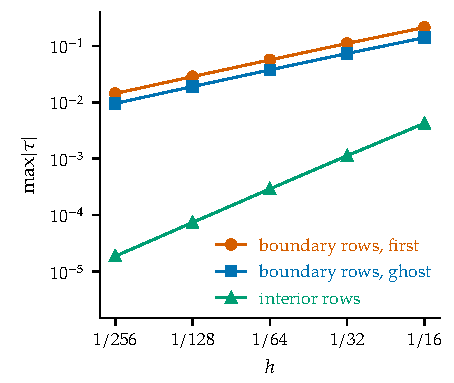
\includegraphics[width=0.48\textwidth]{figures/truncation.pdf}
\caption{Truncation error on the Robin variant (source: \texttt{results/mms\_checks.csv}).
Boundary rows of both closures decay like $h$ and interior rows like $h^2$, although the
global orders in Figure~\ref{fig:conv} differ.}
\label{fig:trunc}
\end{figure}

\subsection{Separating algebraic from discretisation error}\label{sec:alg}
\paragraph{Direct solve: residual and forward bound.} For the representative Robin/ghost run
at $N=64$ the scaled residual \eqref{eq:sres} of the direct solve is $\rho=4.4\times10^{-16}$.
Tables~\ref{tab:neu}--\ref{tab:rob} list $\rho$ for every mesh, with largest value
$8.0\times10^{-13}$ (first-order Neumann, $N=256$). Writing $r_{\mathrm{alg}}=F-A\widetilde U$ for
the computed discrete solution $\widetilde U$, and letting $U_h$ denote the exact discrete
solution of $AU=F$, the same comparison functions as in Theorem~\ref{thm:conv} give
\[
\|\widetilde U-U_h\|_\infty
\le\tfrac12\|r_{\mathrm{alg},I}\|_\infty+
\begin{cases}
\|r_{\mathrm{alg},B}\|_\infty,&\text{first-order},\\
\tfrac h2\|r_{\mathrm{alg},B}\|_\infty,&\text{ghost}.
\end{cases}
\]
For this solve $\|r_{\mathrm{alg},I}\|_\infty=4.48\times10^{-11}$ and
$\|r_{\mathrm{alg},B}\|_\infty=2.77\times10^{-11}$ (rows scaled by $h^{-2}$), so
$\|\widetilde U-U_h\|_\infty\le2.26\times10^{-11}$, six orders of magnitude below the
discretisation error $3.34\times10^{-5}$ on this mesh. Independently, a componentwise backward
error $\rho$ bounds the normwise relative backward error in the $1$-norm by $\rho$, and the
standard perturbation bound $\|\widetilde U-U_h\|_1/\|U_h\|_1\le2\kappa_1(A)\rho/(1-\kappa_1(A)\rho)$
\cite{higham} gives a relative bound of about $3.0\times10^{-12}$, with
$\kappa_1(A)\approx\|A\|_1\|A^{-1}\|_1\approx3.39\times10^3$ estimated by \texttt{onenormest}. The $2$-norm condition number of the symmetrised matrix $DA$, estimated
from the extreme eigenvalues via \texttt{eigsh}, is $\kappa_2(DA)\approx2.18\times10^3$
($\lambda_{\max}\approx3.27\times10^4$, $\lambda_{\min}\approx15.0$). At $N=128$ and $N=256$
the same estimate gives $8.71\times10^3$ and $3.48\times10^4$, in line with $O(N^2)$ growth.
These values are recorded in \texttt{results/mms\_checks\_log.txt} and
\texttt{results/forward\_error\_bound.csv}.

\paragraph{CG tolerance sweep.} Table~\ref{tab:tolsweep} applies CG to $DA\,U=DF$
(Proposition~\ref{prop:sym}) on the Robin variant at $N=64$, from $U_0=0$, with the residual
stopping rule $\|DF-DA\,U_k\|_2\le\mathrm{tol}\,\|DF\|_2$ and
$\mathrm{tol}=10^{-4},\dots,10^{-12}$ (\texttt{code/run\_tolerance\_sweep.py}). The algebraic
error $\|U_{\mathrm{CG}}-U_{\mathrm{dir}}\|_\infty$ falls roughly in proportion to tol. For the
ghost closure the total error is $1.88\times10^{-3}$ at $\mathrm{tol}=10^{-4}$, about $56$ times
the discretisation error $3.34\times10^{-5}$, and still $17\%$ too large at $10^{-6}$. From
$10^{-8}$ on it agrees with the direct solve to three significant figures. The first-order
closure has a larger discretisation error ($8.36\times10^{-3}$), which hides the algebraic
error from $\mathrm{tol}=10^{-6}$ on (within $0.1\%$). Once the algebraic error is well below the
discretisation level, a tighter tolerance only adds iterations ($243\to309$ for the ghost
closure); the total error no longer decreases, because what remains is truncation error.

\begin{table}[H]\centering\footnotesize
\begin{tabular}{@{}llrcccc@{}}\toprule
Closure & tol & iters & $\|DF-DAU\|_2/\|DF\|_2$ & $\rho$ & $\|U_{\mathrm{CG}}-U_{\mathrm{dir}}\|_\infty$ & $\|U_{\mathrm{CG}}-u^*\|_\infty$\\\midrule
ghost-point & $10^{-4}$ & 147 & $9.21\times10^{-5}$ & $2.54\times10^{-5}$ & $1.88\times10^{-3}$ & $1.883\times10^{-3}$\\
ghost-point & $10^{-6}$ & 193 & $9.97\times10^{-7}$ & $1.61\times10^{-7}$ & $2.05\times10^{-5}$ & $3.894\times10^{-5}$\\
ghost-point & $10^{-8}$ & 243 & $8.60\times10^{-9}$ & $1.32\times10^{-9}$ & $8.60\times10^{-8}$ & $3.337\times10^{-5}$\\
ghost-point & $10^{-10}$ & 282 & $8.23\times10^{-11}$ & $1.80\times10^{-11}$ & $7.47\times10^{-10}$ & $3.335\times10^{-5}$\\
ghost-point & $10^{-12}$ & 309 & $9.20\times10^{-13}$ & $1.80\times10^{-13}$ & $8.83\times10^{-12}$ & $3.335\times10^{-5}$\\
\multicolumn{6}{@{}l}{\quad direct \texttt{spsolve}, same mesh} & $3.335\times10^{-5}$\\
\midrule
first-order & $10^{-4}$ & 148 & $9.09\times10^{-5}$ & $2.84\times10^{-5}$ & $1.79\times10^{-3}$ & $9.438\times10^{-3}$\\
first-order & $10^{-6}$ & 194 & $9.59\times10^{-7}$ & $2.41\times10^{-7}$ & $1.93\times10^{-5}$ & $8.360\times10^{-3}$\\
first-order & $10^{-8}$ & 244 & $9.70\times10^{-9}$ & $3.04\times10^{-9}$ & $1.39\times10^{-7}$ & $8.355\times10^{-3}$\\
first-order & $10^{-10}$ & 281 & $9.45\times10^{-11}$ & $3.00\times10^{-11}$ & $1.61\times10^{-9}$ & $8.355\times10^{-3}$\\
first-order & $10^{-12}$ & 316 & $9.44\times10^{-13}$ & $2.26\times10^{-13}$ & $7.58\times10^{-12}$ & $8.355\times10^{-3}$\\
\multicolumn{6}{@{}l}{\quad direct \texttt{spsolve}, same mesh} & $8.355\times10^{-3}$\\
\bottomrule
\end{tabular}

\caption{CG tolerance sweep on $DA\,U=DF$, Robin variant ($\beta=2$), $N=64$, $U_0=0$.
$\rho$: scaled residual \eqref{eq:sres} of the CG iterate in the unscaled system $AU=F$. The
last row of each block is the direct \texttt{spsolve} on the same mesh.
Source: \texttt{results/tolerance\_sweep.csv}.}
\label{tab:tolsweep}
\end{table}

\paragraph{Selected tolerance and fitted order.} Because $\kappa_2(DA)$ grows like $N^2$, a fixed
relative tolerance leaves an algebraic error that grows under refinement, while the ghost
discretisation error falls like $h^2$. Table~\ref{tab:tolorder} repeats the refinement
$N=16,\dots,256$ (Robin) with CG. At $\mathrm{tol}=10^{-8}$ the ghost error at $N=256$ is
$2.443\times10^{-6}$ instead of $2.085\times10^{-6}$, and the last-pair $L^\infty$ order drops to
$1.78$ (fit $1.95$). At $\mathrm{tol}=10^{-10}$ the errors agree with the direct solve to within
$0.1\%$ (largest deviation $0.094\%$, $2.0831\times10^{-6}$ against $2.0851\times10^{-6}$ at
$N=256$), and the orders are the same ($2.00$). The first-order closure is insensitive at both tolerances. Iteration
counts grow roughly like $N$ ($243$ at $N=64$ and $925$ at $N=256$ for $\mathrm{tol}=10^{-8}$),
consistent with $\sqrt{\kappa_2(DA)}\propto N$. We use $\mathrm{tol}=10^{-10}$ for any CG solve
with $N\le256$; the cross-checks in Section~\ref{sec:impl} use $10^{-12}$. All reported errors
come from \texttt{spsolve}, which has no iterative tolerance, and its residual $\rho$ is listed
in Tables~\ref{tab:neu}--\ref{tab:rob}. The reported rates are therefore discretisation rates.

\begin{table}[H]\centering\footnotesize
\begin{tabular}{@{}llcccc@{}}\toprule
Closure & solver & $\|e\|_\infty$ at $N=256$ & last-pair $p_\infty$ & fit $p_\infty$ & fit $p_{L^2_h}$\\\midrule
ghost-point & direct \texttt{spsolve} & $2.085\times10^{-6}$ & 2.00 & 2.00 & 2.00\\
ghost-point & CG, tol $10^{-8}$ (925 it.) & $2.443\times10^{-6}$ & 1.78 & 1.95 & 1.98\\
ghost-point & CG, tol $10^{-10}$ (1087 it.) & $2.083\times10^{-6}$ & 2.00 & 2.00 & 2.00\\
\midrule
first-order & direct \texttt{spsolve} & $2.075\times10^{-3}$ & 1.00 & 1.01 & 1.02\\
first-order & CG, tol $10^{-8}$ (923 it.) & $2.074\times10^{-3}$ & 1.00 & 1.01 & 1.02\\
first-order & CG, tol $10^{-10}$ (1091 it.) & $2.075\times10^{-3}$ & 1.00 & 1.01 & 1.02\\
\bottomrule
\end{tabular}

\caption{Fitted orders with CG at the selected tolerance, Robin variant, $N=16,\dots,256$
(least-squares fits over all five levels, as in Figure~\ref{fig:conv}; iteration counts at
$N=256$). Source: \texttt{results/tolerance\_order\_check.csv},
\texttt{results/tolerance\_order\_fit.csv}.}
\label{tab:tolorder}
\end{table}

% ============================================================
\section{Numerical Experiments}\label{sec:exp}
% ============================================================
\subsection{Comparison of the two closures}
We refine both variants with both closures and keep every other setting fixed: the grids
$N=16,\dots,256$, the manufactured data \eqref{eq:mms}, the norms $L^2_h$ and nodal
$L^\infty$, and \texttt{spsolve}. The results in Tables~\ref{tab:neu}--\ref{tab:rob} and
Figure~\ref{fig:conv} are the experimental side of Theorem~\ref{thm:conv}.

\begin{table}[H]\centering\scriptsize
\begin{tabular}{@{}llrccccccc@{}}\toprule
Closure & $N$ & $h$ & $\|e\|_{L^2_h}$ & $p$ & $\|e\|_{\infty}$ & $p$ & $\|e\|_{\infty,\Gamma_B}$ & $\|e\|_{\infty,\mathrm{int}}$ & $\rho$\\\midrule
first-order & 16 & 1/16 & $1.786\times10^{-2}$ & --- & $5.832\times10^{-2}$ & --- & $5.832\times10^{-2}$ & $4.863\times10^{-2}$ & $2.3\times10^{-14}$\\
first-order & 32 & 1/32 & $8.515\times10^{-3}$ & 1.07 & $2.815\times10^{-2}$ & 1.05 & $2.815\times10^{-2}$ & $2.574\times10^{-2}$ & $3.2\times10^{-14}$\\
first-order & 64 & 1/64 & $4.161\times10^{-3}$ & 1.03 & $1.383\times10^{-2}$ & 1.03 & $1.383\times10^{-2}$ & $1.322\times10^{-2}$ & $7.7\times10^{-14}$\\
first-order & 128 & 1/128 & $2.058\times10^{-3}$ & 1.02 & $6.853\times10^{-3}$ & 1.01 & $6.853\times10^{-3}$ & $6.701\times10^{-3}$ & $2.4\times10^{-13}$\\
first-order & 256 & 1/256 & $1.023\times10^{-3}$ & 1.01 & $3.411\times10^{-3}$ & 1.01 & $3.411\times10^{-3}$ & $3.373\times10^{-3}$ & $8.0\times10^{-13}$\\
\midrule
ghost-point & 16 & 1/16 & $2.206\times10^{-4}$ & --- & $8.611\times10^{-4}$ & --- & $8.611\times10^{-4}$ & $6.706\times10^{-4}$ & $2.6\times10^{-16}$\\
ghost-point & 32 & 1/32 & $5.499\times10^{-5}$ & 2.00 & $2.163\times10^{-4}$ & 1.99 & $2.163\times10^{-4}$ & $1.914\times10^{-4}$ & $3.1\times10^{-16}$\\
ghost-point & 64 & 1/64 & $1.374\times10^{-5}$ & 2.00 & $5.412\times10^{-5}$ & 2.00 & $5.412\times10^{-5}$ & $5.096\times10^{-5}$ & $3.7\times10^{-16}$\\
ghost-point & 128 & 1/128 & $3.434\times10^{-6}$ & 2.00 & $1.354\times10^{-5}$ & 2.00 & $1.354\times10^{-5}$ & $1.314\times10^{-5}$ & $4.0\times10^{-16}$\\
ghost-point & 256 & 1/256 & $8.584\times10^{-7}$ & 2.00 & $3.385\times10^{-6}$ & 2.00 & $3.385\times10^{-6}$ & $3.334\times10^{-6}$ & $7.2\times10^{-16}$\\
\bottomrule
\end{tabular}
\caption{Neumann variant ($\beta=0$). $\|e\|_{\infty,\GB}$: max error over right-edge nodes;
$\|e\|_{\infty,\mathrm{int}}$: max over the remaining unknowns. Last-pair observed orders
round to $1.01$ (first-order) and $2.00$ (ghost) in both norms, matching Theorem~\ref{thm:conv}.
$\rho$: scaled residual \eqref{eq:sres} of the direct solve (\texttt{spsolve} is a direct method,
so there is no iterative tolerance). Sources: \texttt{results/convergence.csv},
\texttt{results/mms\_checks.csv}.}
\label{tab:neu}
\end{table}
\begin{table}[H]\centering\scriptsize
\begin{tabular}{@{}llrccccccc@{}}\toprule
Closure & $N$ & $h$ & $\|e\|_{L^2_h}$ & $p$ & $\|e\|_{\infty}$ & $p$ & $\|e\|_{\infty,\Gamma_B}$ & $\|e\|_{\infty,\mathrm{int}}$ & $\rho$\\\midrule
first-order & 16 & 1/16 & $1.059\times10^{-2}$ & --- & $3.430\times10^{-2}$ & --- & $3.430\times10^{-2}$ & $2.854\times10^{-2}$ & $3.9\times10^{-15}$\\
first-order & 32 & 1/32 & $5.143\times10^{-3}$ & 1.04 & $1.685\times10^{-2}$ & 1.03 & $1.685\times10^{-2}$ & $1.537\times10^{-2}$ & $1.9\times10^{-14}$\\
first-order & 64 & 1/64 & $2.536\times10^{-3}$ & 1.02 & $8.355\times10^{-3}$ & 1.01 & $8.355\times10^{-3}$ & $7.978\times10^{-3}$ & $6.6\times10^{-14}$\\
first-order & 128 & 1/128 & $1.259\times10^{-3}$ & 1.01 & $4.159\times10^{-3}$ & 1.01 & $4.159\times10^{-3}$ & $4.064\times10^{-3}$ & $2.9\times10^{-13}$\\
first-order & 256 & 1/256 & $6.276\times10^{-4}$ & 1.00 & $2.075\times10^{-3}$ & 1.00 & $2.075\times10^{-3}$ & $2.051\times10^{-3}$ & $5.4\times10^{-13}$\\
\midrule
ghost-point & 16 & 1/16 & $1.273\times10^{-4}$ & --- & $5.307\times10^{-4}$ & --- & $5.307\times10^{-4}$ & $3.928\times10^{-4}$ & $2.5\times10^{-16}$\\
ghost-point & 32 & 1/32 & $3.162\times10^{-5}$ & 2.01 & $1.332\times10^{-4}$ & 1.99 & $1.332\times10^{-4}$ & $1.149\times10^{-4}$ & $3.2\times10^{-16}$\\
ghost-point & 64 & 1/64 & $7.892\times10^{-6}$ & 2.00 & $3.335\times10^{-5}$ & 2.00 & $3.335\times10^{-5}$ & $3.098\times10^{-5}$ & $4.4\times10^{-16}$\\
ghost-point & 128 & 1/128 & $1.972\times10^{-6}$ & 2.00 & $8.340\times10^{-6}$ & 2.00 & $8.340\times10^{-6}$ & $8.039\times10^{-6}$ & $4.7\times10^{-16}$\\
ghost-point & 256 & 1/256 & $4.930\times10^{-7}$ & 2.00 & $2.085\times10^{-6}$ & 2.00 & $2.085\times10^{-6}$ & $2.047\times10^{-6}$ & $7.1\times10^{-16}$\\
\bottomrule
\end{tabular}
\caption{Robin variant ($\beta=2$). Same layout as Table~\ref{tab:neu}; last-pair orders round
to $1.00$ (first-order) and $2.00$ (ghost) in both norms. Absolute errors are smaller than in
the Neumann table for every corresponding entry.}
\label{tab:rob}
\end{table}

\begin{figure}[H]\centering
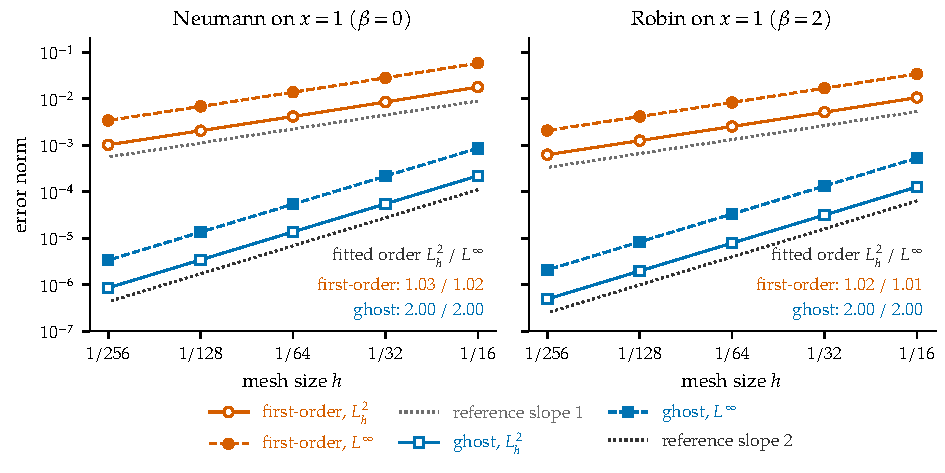
\includegraphics[width=\textwidth]{figures/convergence.pdf}
\caption{Refinement study, $N=16,\dots,256$ (\texttt{results/convergence.csv}), drawn with the course
\texttt{convergence\_plot\_template.py}: measured $L^2_h$ (solid) and $L^\infty$ (dashed) errors with dotted
reference slopes 1 and 2. Each panel prints the least-squares orders over all five levels
($L^2_h$ / $L^\infty$); the largest deviation from the fitted line is $0.016$ in $\ln E$
(\texttt{results/convergence\_fit.csv}). The two-to-one slope ratio confirms that the boundary closure alone sets the global convergence rate.}
\label{fig:conv}
\end{figure}

\paragraph{Interpretation.}
\begin{itemize}[leftmargin=1.5em]
\item From $N=32$ on, every successive pair gives an observed order in $[1.00,1.07]$ for the
first-order closure and in $[1.99,2.01]$ for the ghost closure, and the orders approach $1$ and
$2$ monotonically. Over all five levels the least-squares $L^2_h$ orders are $1.03$ and $2.00$
for Neumann and $1.02$ and $2.00$ for Robin (Figure~\ref{fig:conv}).
\item The maximum error sits on $\GB$ in every run ($\|e\|_{\infty,\GB}=\|e\|_\infty$), near
$y\approx0.6$--$0.7$. For the first-order Neumann run at $N=256$ the interior maximum is
almost as large ($3.37\times10^{-3}$ against $3.41\times10^{-3}$). The $O(h)$ flux defect
spreads through the whole domain, and the global error is set by the closure.
\item The measured errors lie below the residual-based bounds of Theorem~\ref{thm:conv}
(Table~\ref{tab:trunc}). For $u^*=e^{x+y}$ their leading terms are
$\tfrac{e^2}{2}h\approx3.69h$ and $\tfrac{e^2}{4}h^2\approx1.85h^2$. At $N=256$ the first-order
Neumann error $3.41\times10^{-3}$ is below $3.69h\approx1.4\times10^{-2}$, and the ghost Neumann
error $3.38\times10^{-6}$ is below $1.85h^2\approx2.8\times10^{-5}$, by factors of about $4$ and
$8$.
\item Robin errors are smaller than Neumann errors for both closures (ghost, $N=256$:
$2.09\times10^{-6}$ against $3.38\times10^{-6}$), which fits the extra diagonal weight $\beta$ in
the boundary rows.
\end{itemize}

\begin{figure}[H]\centering
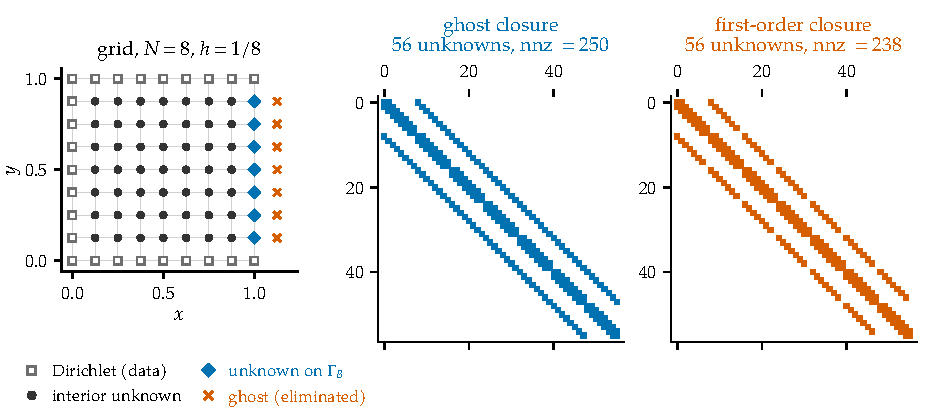
\includegraphics[width=\textwidth]{figures/spy.pdf}
\caption{Left: the $N=8$ grid that the solver resolves---Dirichlet nodes (data, including the four
corners), interior unknowns, the unknowns on $\GB$ and the ghost points $x=1+h$ eliminated by the
ghost closure. Centre and right: sparsity pattern of $A$ on this grid (56 unknowns, lexicographic
order), ghost closure (centre, 250 nonzeros) and first-order closure (right, 238). Both matrices are five-diagonal and banded;
they differ only in the right-edge rows (every eighth row), where the first-order row keeps just
two entries, so the closure changes the matrix only locally. Sparse LU cost also depends on
ordering and fill-in. Measured median \texttt{spsolve} times are reported in Table~\ref{tab:cost}: the cost gap there
comes from needing different $N$ to hit the same error target.}
\label{fig:spy}
\end{figure}

\begin{figure}[H]\centering
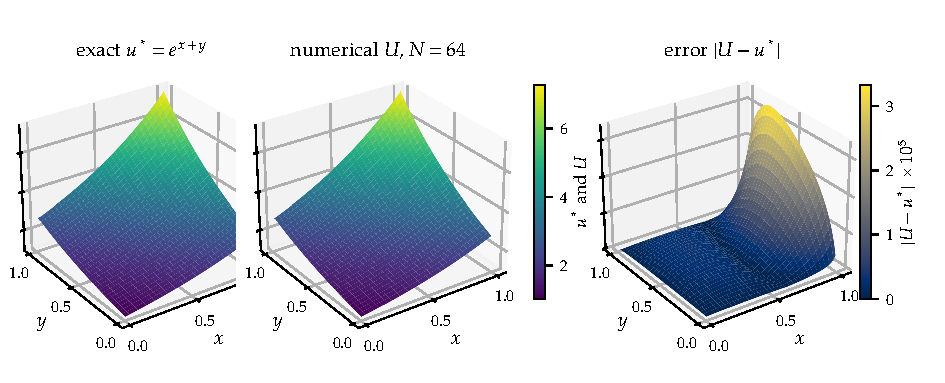
\includegraphics[width=\textwidth]{figures/solution_surface.pdf}
\caption{Solution surface for the Robin variant ($\beta=2$), ghost closure, $N=64$, computed with
\texttt{spsolve}: exact $u^*=e^{x+y}$ (left), numerical $U$ (centre) and pointwise error
$|U-u^*|$ (right). The left and centre surfaces share one colour bar for the solution value $u$;
the error has its own colour bar in units of $10^{-5}$. Arrays follow the solver layout
\texttt{meshgrid(Jg, Ig, indexing="ij")}, so axis~0 is $y$ (index $j$) and axis~1 is $x$
(index $i$). $U$ is visually indistinguishable from $u^*$; the error,
at most $3.34\times10^{-5}$ (attained on $\GB$, $y\approx0.70$), is concentrated on the flux edge
and vanishes towards the Dirichlet edges, consistent with Tables~\ref{tab:neu}--\ref{tab:rob}.
The maximum error and its location are recorded in
\texttt{results/solution\_surface\_log.txt}.}
\label{fig:surface}
\end{figure}

\subsection{Cost versus accuracy}
We compare the closures at the accuracy target $\|e\|_\infty\le5\times10^{-3}$, chosen so that
both reach it with $N\le512$. The ghost closure already meets a tighter target of $10^{-3}$ at
$N=16$, but at $N=512$ the first-order closure still has $\|e\|_\infty=1.70\times10^{-3}$
(Neumann) and $1.036\times10^{-3}$ (Robin), as recorded in
\texttt{results/cost\_accuracy\_all.csv}. Cost is the median wall time of \texttt{spsolve} over
five runs after one warm-up solve. The min--max range of the five runs is given in
Table~\ref{tab:cost} and drawn as horizontal bars in Figure~\ref{fig:cost}. For the four
matched-target runs all five times lie within $\CostSpreadMatched\%$ of the median. Over all
$24$ runs the largest single time is $\CostWorstRatio$ times the median (\CostWorstCase), which
is why we use the median and not the mean. The timing covers the sparse LU factorisation and
the triangular solves inside \texttt{spsolve}. It leaves out matrix assembly, data evaluation,
I/O, the CG cross-check, figure rendering and Python overhead outside \texttt{spsolve}.
Assembly is an $O(M)$ step for either closure and was not timed. The measured values are in
Table~\ref{tab:cost} and Figure~\ref{fig:cost}, from \texttt{results/cost\_accuracy.csv}.

\begin{table}[H]\centering\small
\begin{tabular}{@{}llrrccc@{}}\toprule
BC & Closure & $N_\mathrm{min}$ & unknowns & $\|e\|_\infty$ & median time (s) & min--max (s)\\\midrule
Neumann & first-order & 256 & 65280 & $3.411\times10^{-3}$ & $2.317\times10^{-1}$ & $(2.28$--$2.43)\times10^{-1}$\\
Neumann & ghost-point & 16 & 240 & $8.611\times10^{-4}$ & $3.261\times10^{-4}$ & $(3.11$--$3.31)\times10^{-4}$\\
Robin & first-order & 128 & 16256 & $4.159\times10^{-3}$ & $3.642\times10^{-2}$ & $(3.63$--$3.86)\times10^{-2}$\\
Robin & ghost-point & 16 & 240 & $5.307\times10^{-4}$ & $3.522\times10^{-4}$ & $(3.18$--$4.02)\times10^{-4}$\\
\bottomrule\end{tabular}

\caption{Smallest tested $N$ reaching $\|e\|_\infty\le5\times10^{-3}$, with measured median
\texttt{spsolve} time over five runs and the min--max range of those runs. Ghost-point needs
$N=16$ in both variants; first-order needs $N=128$ (Robin) or $N=256$ (Neumann). The solve-time
ratio is about $10^{2}$--$10^{3}$. Times are machine-dependent (single machine); only the ratio
is interpreted.}
\label{tab:cost}
\end{table}

\begin{figure}[H]\centering
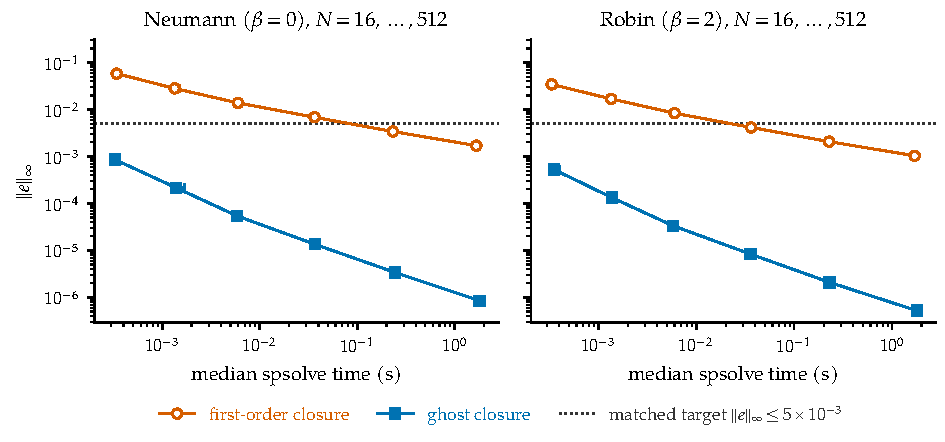
\includegraphics[width=\textwidth]{figures/cost_accuracy.pdf}
\caption{Error against measured median \texttt{spsolve} time for both closures and both
variants, $N=16,\dots,512$ (source: \texttt{results/cost\_accuracy\_all.csv}); horizontal bars
span the minimum and maximum of the five timed runs. The dotted line is the matched accuracy
target $\|e\|_\infty\le5\times10^{-3}$ of Table~\ref{tab:cost}, stated on the figure.
Ghost runs (squares) already meet the target at $N=16$; first-order runs (circles) need
$N=128$ (Robin) or $N=256$ (Neumann), so the same accuracy costs two to three orders of
magnitude more wall time. At matched accuracy the cost is set by the global order, not by the
simplicity of the boundary row.}
\label{fig:cost}
\end{figure}

\subsection{Pure-Neumann problem (not attempted)}
The Problem Pack lists a pure-Neumann variant as optional depth. It would need the
compatibility condition, a constant null vector and a gauge fix. We did not attempt it, and
Remark~\ref{rem:beta} records the theory that such a study would test.

\subsection{Incompatible data at the mixed corner}\label{sec:incompat}
On the unit square the mixed corner has opening $\omega=\pi/2$, and the Dirichlet--Neumann
exponents are the odd integers $\lambda=1,3,5,\dots$ (Section~\ref{sec:model}). With smooth
compatible data the formal $r^\lambda$ modes are harmonic polynomials, for instance
$r\sin\theta=y$, and no genuine singularity appears. The manufactured solution \eqref{eq:mms}
is entire and compatible, so the baseline experiment cannot see a corner effect. Incompatible
data at the mixed corner bring in the $r\log r$ companion of the $\lambda=1$ mode. The $C^4$
hypothesis of the comparison-function argument then fails, and Theorem~\ref{thm:conv} does not
apply to this case.

To test this situation we keep the domain $\Omega=(0,1)^2$, the five-point stencil, the two
closures \eqref{eq:first}--\eqref{eq:ghost} and the Dirichlet treatment of all four corners, and
change only the manufactured solution. At the mixed corner $(1,0)$ let
$z=(1-x)+\mathrm{i}y$, $r=|z|$ and $\theta=\mathrm{atan2}(y,1-x)\in[0,\pi/2]$. Here $r$ denotes the
distance to $(1,0)$, distinct from the Robin datum $r$ in~\eqref{eq:bvp}. We set
\begin{equation}\label{eq:mmsinc}
u^*(x,y)=\mathrm{Im}(z\,\mathrm{Log}\,z)=y\log r+(1-x)\theta.
\end{equation}
The function is harmonic for $r>0$ (so $f=0$), with a singularity only at $(1,0)$; near
$(1,1)$ and the other two corners it is smooth. All boundary data are induced from $u^*$:
$g=u^*$ on $\GD$, and the flux data on $\GB$ are
$r_{\mathrm{bdry}}=\partial_n u^*+\beta u^*=u_x+\beta u^*$. The identities $u_x=-\theta$ and,
on $x=1$ with $y>0$, $u^*=y\log y$ give $r_{\mathrm{bdry}}(y)=-\pi/2+\beta y\log y$; for the
Neumann variant this is the constant $-\pi/2$. At $(1,0)$ one has $r\log r\to0$, so
$g(1,0)=0$ is assigned directly and $\log 0$ is never evaluated. The same data are compatible
at $(1,1)$: both the Dirichlet trace along $y=1$ and the flux law on $x=1$ give
$u_x(1,1)=-\pi/2$. The incompatibility is at $(1,0)$ only. If $u$ were $C^1$ up to that
corner, $u=0$ on $y=0$ would force $u_x(1,0)=0$, but the flux data equal $-\pi/2$. The
function \eqref{eq:mmsinc} has the form of the resonant companion of the
$\lambda=1$ mode at this mixed right angle \cite{grisvard}. First derivatives are already
unbounded ($u_y=1+\log r$), and $u_{xx}=-y/r^2=O(1/r)$, so $u^*\notin H^2(\Omega)$ and the
$C^4$ assumption of Theorem~\ref{thm:conv} fails.

Because Theorem~\ref{thm:conv} no longer applies, we examine these questions numerically. The
assembly, the two closures and the discrete norms $L^2_h$ and nodal $L^\infty$ are those of
the main experiment, on the meshes $N=16,32,64,128,256$ and one finer mesh $N=512$. We record
where the nodal maximum sits and split the error at the radius $r=1/4$ from $(1,0)$, with
$r<1/4$ as the near region and $r\ge 1/4$ as the far region. The split at $r=1/4$ is chosen a
priori on geometric grounds. Both the Neumann ($\beta=0$) and Robin
($\beta=2$) variants are run. We ask whether the observed orders drop, whether the ghost
closure remains one order higher, and whether the maximum error concentrates at the mixed
corner.

\begin{table}[H]\centering\scriptsize
\begin{tabular}{@{}llrcccccc@{}}\toprule
Closure & $N$ & $h$ & $\|e\|_{L^2_h}$ & $p$ & $\|e\|_{\infty}$ & $p$ & $\|e\|_{\infty,\Gamma_B}$ & $\|e\|_{\infty,\mathrm{int}}$\\\midrule
first-order & 16 & 1/16 & $1.169\times10^{-2}$ & --- & $5.406\times10^{-2}$ & --- & $5.406\times10^{-2}$ & $3.370\times10^{-2}$\\
first-order & 32 & 1/32 & $5.651\times10^{-3}$ & 1.05 & $2.761\times10^{-2}$ & 0.97 & $2.761\times10^{-2}$ & $1.903\times10^{-2}$\\
first-order & 64 & 1/64 & $2.778\times10^{-3}$ & 1.02 & $1.395\times10^{-2}$ & 0.98 & $1.395\times10^{-2}$ & $1.032\times10^{-2}$\\
first-order & 128 & 1/128 & $1.377\times10^{-3}$ & 1.01 & $7.013\times10^{-3}$ & 0.99 & $7.013\times10^{-3}$ & $5.444\times10^{-3}$\\
first-order & 256 & 1/256 & $6.855\times10^{-4}$ & 1.01 & $3.516\times10^{-3}$ & 1.00 & $3.516\times10^{-3}$ & $2.823\times10^{-3}$\\
first-order & 512 & 1/512 & $3.420\times10^{-4}$ & 1.00 & $1.760\times10^{-3}$ & 1.00 & $1.760\times10^{-3}$ & $1.447\times10^{-3}$\\
\midrule
ghost-point & 16 & 1/16 & $7.610\times10^{-4}$ & --- & $1.050\times10^{-2}$ & --- & $1.050\times10^{-2}$ & $3.040\times10^{-3}$\\
ghost-point & 32 & 1/32 & $2.126\times10^{-4}$ & 1.84 & $5.261\times10^{-3}$ & 1.00 & $5.261\times10^{-3}$ & $1.541\times10^{-3}$\\
ghost-point & 64 & 1/64 & $5.821\times10^{-5}$ & 1.87 & $2.632\times10^{-3}$ & 1.00 & $2.632\times10^{-3}$ & $7.732\times10^{-4}$\\
ghost-point & 128 & 1/128 & $1.572\times10^{-5}$ & 1.89 & $1.316\times10^{-3}$ & 1.00 & $1.316\times10^{-3}$ & $3.869\times10^{-4}$\\
ghost-point & 256 & 1/256 & $4.200\times10^{-6}$ & 1.90 & $6.580\times10^{-4}$ & 1.00 & $6.580\times10^{-4}$ & $1.935\times10^{-4}$\\
ghost-point & 512 & 1/512 & $1.114\times10^{-6}$ & 1.92 & $3.290\times10^{-4}$ & 1.00 & $3.290\times10^{-4}$ & $9.676\times10^{-5}$\\
\bottomrule
\end{tabular}

\caption{Incompatible data \eqref{eq:mmsinc}, Neumann variant ($\beta=0$). Same norms as
Table~\ref{tab:neu}. Last-pair observed orders ($N=256$ to $N=512$) are $1.00$ in both
norms for the first-order closure, and $1.92$ ($L^2_h$) / $1.00$ ($L^\infty$) for the
ghost closure. In every row $\|e\|_{\infty,\GB}=\|e\|_\infty$. Source:
\texttt{results/incompatible\_convergence.csv}.}
\label{tab:incneu}
\end{table}
\begin{table}[H]\centering\scriptsize
\begin{tabular}{@{}lrcccccc@{}}\toprule
Closure & $N$ & $\|e\|_{\infty,\mathrm{near}}$ & $p$ & $\|e\|_{\infty,\mathrm{far}}$ & $p$ & $(x,y)_{\max}$ & $r_{\max}$\\\midrule
first-order & 16 & $5.406\times10^{-2}$ & --- & $4.102\times10^{-2}$ & --- & $(1,h)$ & $h$\\
first-order & 32 & $2.761\times10^{-2}$ & 0.97 & $2.014\times10^{-2}$ & 1.03 & $(1,h)$ & $h$\\
first-order & 64 & $1.395\times10^{-2}$ & 0.98 & $9.980\times10^{-3}$ & 1.01 & $(1,h)$ & $h$\\
first-order & 128 & $7.013\times10^{-3}$ & 0.99 & $4.968\times10^{-3}$ & 1.01 & $(1,h)$ & $h$\\
first-order & 256 & $3.516\times10^{-3}$ & 1.00 & $2.478\times10^{-3}$ & 1.00 & $(1,h)$ & $h$\\
first-order & 512 & $1.760\times10^{-3}$ & 1.00 & $1.238\times10^{-3}$ & 1.00 & $(1,h)$ & $h$\\
\midrule
ghost-point & 16 & $1.050\times10^{-2}$ & --- & $2.580\times10^{-3}$ & --- & $(1,h)$ & $h$\\
ghost-point & 32 & $5.261\times10^{-3}$ & 1.00 & $6.270\times10^{-4}$ & 2.04 & $(1,h)$ & $h$\\
ghost-point & 64 & $2.632\times10^{-3}$ & 1.00 & $1.559\times10^{-4}$ & 2.01 & $(1,h)$ & $h$\\
ghost-point & 128 & $1.316\times10^{-3}$ & 1.00 & $3.892\times10^{-5}$ & 2.00 & $(1,h)$ & $h$\\
ghost-point & 256 & $6.580\times10^{-4}$ & 1.00 & $9.726\times10^{-6}$ & 2.00 & $(1,h)$ & $h$\\
ghost-point & 512 & $3.290\times10^{-4}$ & 1.00 & $2.431\times10^{-6}$ & 2.00 & $(1,h)$ & $h$\\
\bottomrule
\end{tabular}

\caption{Same Neumann runs as Table~\ref{tab:incneu}, split at the fixed radius $r=1/4$
from $(1,0)$. Near: $r<1/4$; far: $r\ge 1/4$. In every computed run the nodal maximum is
attained at the nearest unknown $(1,h)$ on $\GB$, so $r_{\max}=h$. Last-pair far-field
orders are $1.00$ (first-order) and $2.00$ (ghost).}
\label{tab:incneusplit}
\end{table}
\begin{table}[H]\centering\scriptsize
\begin{tabular}{@{}llrcccccc@{}}\toprule
Closure & $N$ & $h$ & $\|e\|_{L^2_h}$ & $p$ & $\|e\|_{\infty}$ & $p$ & $\|e\|_{\infty,\Gamma_B}$ & $\|e\|_{\infty,\mathrm{int}}$\\\midrule
first-order & 16 & 1/16 & $7.247\times10^{-3}$ & --- & $4.249\times10^{-2}$ & --- & $4.249\times10^{-2}$ & $2.293\times10^{-2}$\\
first-order & 32 & 1/32 & $3.563\times10^{-3}$ & 1.02 & $2.393\times10^{-2}$ & 0.83 & $2.393\times10^{-2}$ & $1.410\times10^{-2}$\\
first-order & 64 & 1/64 & $1.763\times10^{-3}$ & 1.02 & $1.284\times10^{-2}$ & 0.90 & $1.284\times10^{-2}$ & $8.198\times10^{-3}$\\
first-order & 128 & 1/128 & $8.762\times10^{-4}$ & 1.01 & $6.689\times10^{-3}$ & 0.94 & $6.689\times10^{-3}$ & $4.578\times10^{-3}$\\
first-order & 256 & 1/256 & $4.368\times10^{-4}$ & 1.00 & $3.424\times10^{-3}$ & 0.97 & $3.424\times10^{-3}$ & $2.478\times10^{-3}$\\
first-order & 512 & 1/512 & $2.181\times10^{-4}$ & 1.00 & $1.734\times10^{-3}$ & 0.98 & $1.734\times10^{-3}$ & $1.313\times10^{-3}$\\
\midrule
ghost-point & 16 & 1/16 & $5.663\times10^{-4}$ & --- & $9.317\times10^{-3}$ & --- & $9.317\times10^{-3}$ & $2.246\times10^{-3}$\\
ghost-point & 32 & 1/32 & $1.664\times10^{-4}$ & 1.77 & $4.930\times10^{-3}$ & 0.92 & $4.930\times10^{-3}$ & $1.299\times10^{-3}$\\
ghost-point & 64 & 1/64 & $4.737\times10^{-5}$ & 1.81 & $2.543\times10^{-3}$ & 0.95 & $2.543\times10^{-3}$ & $7.047\times10^{-4}$\\
ghost-point & 128 & 1/128 & $1.318\times10^{-5}$ & 1.85 & $1.293\times10^{-3}$ & 0.98 & $1.293\times10^{-3}$ & $3.685\times10^{-4}$\\
ghost-point & 256 & 1/256 & $3.605\times10^{-6}$ & 1.87 & $6.521\times10^{-4}$ & 0.99 & $6.521\times10^{-4}$ & $1.887\times10^{-4}$\\
ghost-point & 512 & 1/512 & $9.735\times10^{-7}$ & 1.89 & $3.275\times10^{-4}$ & 0.99 & $3.275\times10^{-4}$ & $9.552\times10^{-5}$\\
\bottomrule
\end{tabular}

\caption{Incompatible data \eqref{eq:mmsinc}, Robin variant ($\beta=2$). Last-pair orders
are $1.00$ ($L^2_h$) / $0.98$ ($L^\infty$) for the first-order closure, and $1.89$ /
$0.99$ for the ghost closure. Source: \texttt{results/incompatible\_convergence.csv}.}
\label{tab:incrob}
\end{table}
\begin{table}[H]\centering\scriptsize
\begin{tabular}{@{}lrcccccc@{}}\toprule
Closure & $N$ & $\|e\|_{\infty,\mathrm{near}}$ & $p$ & $\|e\|_{\infty,\mathrm{far}}$ & $p$ & $(x,y)_{\max}$ & $r_{\max}$\\\midrule
first-order & 16 & $4.249\times10^{-2}$ & --- & $2.549\times10^{-2}$ & --- & $(1,h)$ & $h$\\
first-order & 32 & $2.393\times10^{-2}$ & 0.83 & $1.278\times10^{-2}$ & 1.00 & $(1,h)$ & $h$\\
first-order & 64 & $1.284\times10^{-2}$ & 0.90 & $6.405\times10^{-3}$ & 1.00 & $(1,h)$ & $h$\\
first-order & 128 & $6.689\times10^{-3}$ & 0.94 & $3.206\times10^{-3}$ & 1.00 & $(1,h)$ & $h$\\
first-order & 256 & $3.424\times10^{-3}$ & 0.97 & $1.604\times10^{-3}$ & 1.00 & $(1,h)$ & $h$\\
first-order & 512 & $1.734\times10^{-3}$ & 0.98 & $8.022\times10^{-4}$ & 1.00 & $(1,h)$ & $h$\\
\midrule
ghost-point & 16 & $9.317\times10^{-3}$ & --- & $1.583\times10^{-3}$ & --- & $(1,h)$ & $h$\\
ghost-point & 32 & $4.930\times10^{-3}$ & 0.92 & $3.793\times10^{-4}$ & 2.06 & $(1,h)$ & $h$\\
ghost-point & 64 & $2.543\times10^{-3}$ & 0.95 & $9.459\times10^{-5}$ & 2.00 & $(1,h)$ & $h$\\
ghost-point & 128 & $1.293\times10^{-3}$ & 0.98 & $2.356\times10^{-5}$ & 2.01 & $(1,h)$ & $h$\\
ghost-point & 256 & $6.521\times10^{-4}$ & 0.99 & $5.884\times10^{-6}$ & 2.00 & $(1,h)$ & $h$\\
ghost-point & 512 & $3.275\times10^{-4}$ & 0.99 & $1.474\times10^{-6}$ & 2.00 & $(1,h)$ & $h$\\
\bottomrule
\end{tabular}

\caption{Robin split companion to Table~\ref{tab:incrob}, same $r=1/4$ partition. The
nodal maximum is again at $(1,h)$ in every run. Last-pair far-field orders are $1.00$
(first-order) and $2.00$ (ghost).}
\label{tab:incrobsplit}
\end{table}

\begin{figure}[H]\centering
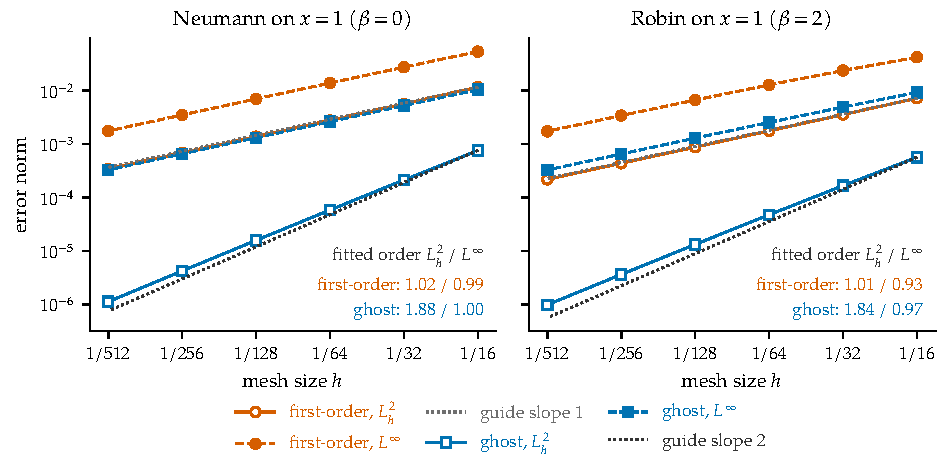
\includegraphics[width=\textwidth]{figures/incompatible-convergence.pdf}
\caption{Incompatible-data refinement study, $N=16,\dots,512$
(\texttt{results/incompatible\_convergence.csv}): measured $L^2_h$ (solid) and $L^\infty$
(dashed) errors. Dotted lines are visual guides of slopes $1$ and $2$ (the smooth-baseline
orders). Least-squares fits over all six levels
give $L^2_h$ orders $1.02$/$1.88$ (Neumann, first/ghost) and $1.01$/$1.84$ (Robin); the
corresponding $L^\infty$ fits are $0.99$/$1.00$ and $0.93$/$0.97$. Over the a-priori
window $N\ge 64$ the $L^2_h$ fits are $1.01$/$1.90$ (Neumann) and $1.00$/$1.87$ (Robin),
and the $L^\infty$ fits are $1.00$/$1.00$ and $0.96$/$0.99$. All fits:
\texttt{results/incompatible\_convergence\_fit.csv}. Corner incompatibility cuts the ghost closure's global $L^\infty$ rate from 2 to 1 while keeping its $L^2_h$ rate near 1.9.}
\label{fig:incconv}
\end{figure}

\begin{figure}[H]\centering
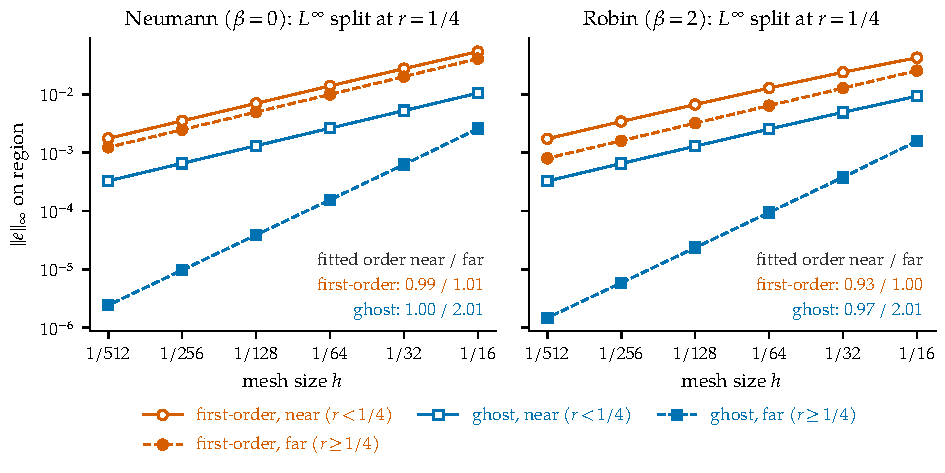
\includegraphics[width=\textwidth]{figures/incompatible-split.pdf}
\caption{Nodal $L^\infty$ error split at the fixed radius $r=1/4$ from $(1,0)$. For both
variants the first-order closure is close to order $1$ in both regions. The ghost closure
is close to order $1$ near the mixed corner and close to order $2$ on $r\ge 1/4$
(Neumann far-field fit $2.01$ over all levels and $2.00$ on $N\ge 64$; Robin $2.01$ and
$2.00$). The global $L^\infty$ order alone would suggest that the ghost closure drops to first
order everywhere, whereas on the tested meshes the loss stays in the corner region and the
far-field error keeps the smooth-data rate.}
\label{fig:incsplit}
\end{figure}

\begin{figure}[H]\centering
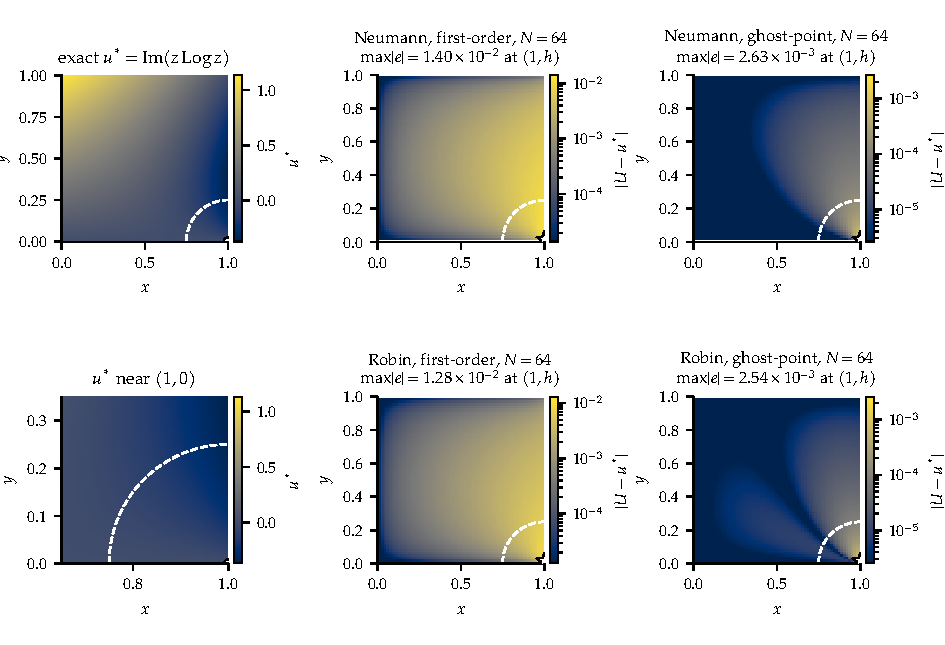
\includegraphics[width=\textwidth]{figures/incompatible-error-field.pdf}
\caption{Exact $u^*$ from \eqref{eq:mmsinc} (left; the function vanishes at $(1,0)$,
where the singularity is in the derivatives) and nodal errors $|U-u^*|$ at $N=64$ for
both closures and both variants (log colour scale; the dashed arc is $r=1/4$; the star
marks the nodal maximum). In every panel the maximum sits at $(1,h)$ on $\GB$. The
first-order error spreads well into the domain; the ghost error is concentrated at the
mixed corner. Source: \texttt{results/incompatible\_fields\_log.txt}.}
\label{fig:incfield}
\end{figure}

\paragraph{Observations.}
\begin{itemize}[leftmargin=1.5em]
\item For the first-order closure the observed global orders remain close to $1$ in both
norms and both variants (Neumann last-pair $1.00$/$1.00$ in $L^2_h$/$L^\infty$; Robin
$1.00$/$0.98$). The same holds in the near and far regions (Tables~\ref{tab:incneusplit} and~\ref{tab:incrobsplit}). The Robin global $L^\infty$
approaches $1$ more slowly, with fits $0.93$ over all six levels and $0.96$ on $N\ge 64$.
\item For the ghost closure the global $L^\infty$ order drops to $1$ (Neumann last-pair
and both fitted windows all round to $1.00$; Robin last-pair $0.99$, fit $0.97$ over all
levels and $0.99$ on $N\ge 64$). The near-corner $L^\infty$ coincides with the global
maximum and follows the same order. On $r\ge 1/4$, however, the ghost $L^\infty$ remains
close to order $2$ (last-pair $2.00$ in both variants). The global $L^2_h$ orders lie between
$1$ and $2$ (Neumann: last pair $1.92$, fits $1.88$/$1.90$; Robin: $1.89$, $1.84$/$1.87$). For
Neumann this is consistent with $h^2|\log h|^{1/2}$, since
$\|e\|_{L^2_h}/(h^2\sqrt{\ln N})\approx0.117$ for every $N$ from $16$ to $512$. The Robin ratio
grows from $0.087$ to $0.102$ and has not yet levelled off. The Neumann data also give
$N\|e\|_\infty\approx0.168$ and, for $N\ge32$, $N^2\|e\|_{\infty,\mathrm{far}}\approx0.64$. A
near-corner profile $|e|\approx Ch^2/r$ would explain all three scalings (the scalings, not the
constants); we have not proved it.
\item In all $24$ runs the nodal maximum is attained at the nearest unknown $(1,h)$ on
$\GB$, at distance $h$ from the mixed corner. Absolute ghost errors remain smaller than
the first-order errors at the same $N$ (Neumann, $N=256$: $6.58\times10^{-4}$ versus
$3.516\times10^{-3}$ in $L^\infty$), but the ghost closure is no longer one full order
higher in the global max-norm. No rate is claimed for this case.
\end{itemize}

\Needspace{14\baselineskip}
\paragraph{What the comparison-function argument can still explain.}
The proof of Theorem~\ref{thm:conv} bounds $\|e\|_\infty$ by a comparison function built
from the residual $\tau=Au^*_h-F$, after Taylor expansions have produced
$\tau_I=O(h^2)$ and $\tau_B=O(h)$ under a $C^4$ assumption. Here those expansions are not
available, but $\tau$ can still be computed as the residual of the grid function. The
interior rows are the same for both closures, and so is their residual: its maximum sits at
$(1-h,h)$ and equals about $0.079/h$, for example $1.2686$ at $N=16$. Substituting
\eqref{eq:mmsinc} into the first-order row at $(1,h)$ gives the $h$-independent value
$\pi/4-\frac12\log 2\approx0.439$, so for that closure the maximum $|\tau|$ is the interior
one.
Substituting into the ghost row at $(1,h)$ gives
$(\pi/2-3\log 2)/h\approx-0.509/h$. Since $0.509/h>0.079/h$, this boundary value is the nodal
maximum of $|\tau|$ for the ghost closure. These residual values are the same for the
Neumann ($\beta=0$) and Robin ($\beta=2$) variants: on $\GB$ one has $u^*=y\log y$ and
$r_{\mathrm{bdry}}=-\pi/2+\beta y\log y$, so the $\beta$ terms cancel exactly in both boundary
rows, and interior rows contain no $\beta$. The computed residuals in
\texttt{results/incompatible\_convergence.csv} agree for the two variants to round-off.
A formal comparison bound driven by these residuals cannot give even a vanishing bound for
the ghost closure, let alone an $O(h^2)$ one: the $(1,h)$ ghost residual alone contributes a non-vanishing $O(1)$ term
$\frac12\bigl|\pi/2-3\log 2\bigr|\approx0.254$. If one also inserts the computed
$\|\tau_I\|_\infty\approx0.079/h$, the same formal bound diverges, so it does not explain
why the observed global $L^\infty$ error still vanishes at a rate close to $1$.
On $r\ge 1/4$ the computed ghost residual shrinks at an observed rate close to $2$, which
matches the far-field errors in Tables~\ref{tab:incneusplit} and~\ref{tab:incrobsplit}. The
rate-2 residual comes from a cancellation in this $u^*$: $u_{xxx}=-2(1-x)y/r^4$ vanishes on
$x=1$, so the $O(h)$ term of \eqref{eq:tauB2} is zero along $\GB$, just as in P1 and P4 for the
first-order closure. Smooth data still give second-order far-field error even when the boundary
residual is $O(h)$; the matching rates here are a consistency check.
The scaled residuals \eqref{eq:sres} of the computed direct solves are at most
$1.9\times10^{-12}$ (Robin, first-order, $N=512$; Neumann, first-order, $N=512$:
$1.5\times10^{-12}$) and at most $4.0\times10^{-15}$ for the ghost closure, far too small to
affect the observed orders.

\subsection{Limitations}
The refinement and cost studies use $u^*=e^{x+y}$ on the unit square, and
Theorem~\ref{thm:conv} is proved under a $C^4$ assumption with constant $\beta\ge 0$. The
course-bank problems of Section~\ref{sec:verif} (five items, four of them independent problems)
include one run with $a=1+x$; variable coefficients and a non-constant $\beta$ are not analysed.
For the incompatible data of Section~\ref{sec:incompat}, and for $\beta<0$, the $O(h)$ and
$O(h^2)$ bounds are not claimed, and the optional pure-Neumann problem was not run
(Remark~\ref{rem:beta}). Timings come from a single machine and count only \texttt{spsolve};
only the ratio between closures is interpreted. Even in the extended cost sweep up to $N=512$
the first-order closure never reaches $10^{-3}$ ($1.70\times10^{-3}$ Neumann,
$1.036\times10^{-3}$ Robin). The comparison-function bounds are rigorous but not sharp, and why
the Robin errors are smaller than the Neumann ones on the smooth baseline has not been analysed.

% ============================================================
\clearpage
\section{Conclusions}\label{sec:concl}
% ============================================================
\begin{itemize}[leftmargin=2em]
\item Both closures have the same $O(h)$ local defect on $\GB$ (Table~\ref{tab:trunc}), yet they
converge globally at orders $1$ and $2$. Theorem~\ref{thm:conv} proves maximum-norm bounds of
these orders with M-matrix comparison functions; the last-pair observed orders in
Tables~\ref{tab:neu}--\ref{tab:rob} are about $1.00$--$1.01$ and $2.00$ in $L^2_h$ and
$L^\infty$ for $N$ up to $256$.
\item In the first-order scheme the closure, not the interior stencil, limits the global
accuracy: at $N=256$ the interior max-norm error is almost as large as the boundary one
(Tables~\ref{tab:neu}--\ref{tab:rob}).
\item Both assembled matrices are nonsymmetric ($\eta(A)\approx0.02$--$0.08$), but a diagonal
scaling of the boundary rows makes $DA$ symmetric positive definite
(Proposition~\ref{prop:sym}), so CG is applied to $DAU=DF$; at $\mathrm{tol}=10^{-10}$ it
matches the direct solve to within $0.1\%$ with the same fitted orders (Section~\ref{sec:alg}).
\item At the matched target $\|e\|_\infty\le5\times10^{-3}$ the ghost closure reaches the tolerance
at $N=16$. Among the tested grids the first-order closure needs $N=128$ (Robin) or $N=256$
(Neumann), and the median \texttt{spsolve} times then differ by two to three orders of
magnitude (Table~\ref{tab:cost}).
\item With incompatible data at the mixed corner, using the exact solution
\eqref{eq:mmsinc}, the first-order closure still shows observed order $1$ in both norms; the
Robin $L^\infty$ last-pair order is $0.98$. The ghost closure drops to order $1$ in global
$L^\infty$, with the maximum at $(1,h)$, while its far-field $L^\infty$ stays close to order
$2$ (Section~\ref{sec:incompat}). These are observations on $N\le 512$;
Theorem~\ref{thm:conv} does not apply.
\end{itemize}

\noindent For rows~\eqref{eq:first}--\eqref{eq:ghost} and $u^*=e^{x+y}$, the ghost closure is the
better choice. Tables~\ref{tab:neu}--\ref{tab:rob} show orders $1$ and $2$, consistent with the
upper bounds of Theorem~\ref{thm:conv} (we have no matching lower bounds), and the ghost closure
reaches the error target at the lower measured solve cost (Table~\ref{tab:cost}). The
first-order closure can still look second order when its leading boundary defect vanishes, as
in the cancellation cases of Section~\ref{sec:verif}.

% ============================================================
\begin{thebibliography}{99}
\bibitem{incropera} T.~L. Bergman, A.~S. Lavine, F.~P. Incropera and D.~P. DeWitt.
\emph{Fundamentals of Heat and Mass Transfer}, 7th ed. John Wiley \& Sons, Hoboken, NJ, 2011.
\bibitem{gresho} P.~M. Gresho and R.~L. Sani. On pressure boundary conditions for the incompressible
Navier--Stokes equations. \emph{International Journal for Numerical Methods in Fluids}
7,~10 (1987), 1111--1145.
\bibitem{evans} L.~C. Evans. \emph{Partial Differential Equations}, 2nd ed. Graduate Studies in
Mathematics~19. American Mathematical Society, Providence, RI, 2010.
\bibitem{grisvard} P.~Grisvard. \emph{Elliptic Problems in Nonsmooth Domains}. Pitman Advanced
Publishing Program, Boston, 1985 (Monographs and Studies in Mathematics~24); reprinted as SIAM
Classics in Applied Mathematics~69, Philadelphia, 2011.
\bibitem{leveque} R.~J. LeVeque. \emph{Finite Difference Methods for Ordinary and Partial Differential
Equations: Steady-State and Time-Dependent Problems}. SIAM, Philadelphia, 2007.
\bibitem{varga} R.~S. Varga. \emph{Matrix Iterative Analysis}, 2nd revised and expanded ed.
Springer Series in Computational Mathematics~27. Springer, Berlin, 2000.
\bibitem{morton} K.~W. Morton and D.~F. Mayers. \emph{Numerical Solution of Partial Differential
Equations: An Introduction}, 2nd ed. Cambridge University Press, 2005.
\bibitem{numpy} C.~R. Harris et al. Array programming with NumPy. \emph{Nature} 585 (2020), 357--362.
\bibitem{matplotlib} J.~D. Hunter. Matplotlib: a 2D graphics environment. \emph{Computing in Science
\& Engineering} 9,~3 (2007), 90--95.
\bibitem{scipy} P.~Virtanen et al. SciPy 1.0: fundamental algorithms for scientific computing in Python.
\emph{Nature Methods} 17 (2020), 261--272.
\bibitem{higham} N.~J. Higham. \emph{Accuracy and Stability of Numerical Algorithms}, 2nd ed. SIAM,
Philadelphia, 2002.

\end{thebibliography}
% Bibliography editions/years verified 2026-11-03 via publisher/DOI pages (LeVeque SIAM 2007;
% Morton--Mayers CUP 2nd ed.\ 2005; Evans AMS GSM~19, 2010; Grisvard
% Pitman 1985 / SIAM Classics~69, 2011; Varga Springer 2000; Bergman et al.\ Wiley 2011;
% Gresho--Sani IJNMF 7 (1987) 1111--1145; Hunter CiSE 9(3) (2007) 90--95; Higham SIAM 2nd ed.\ 2002). Section pointers are to the standard chapter locations;
% hand-check against the physical/library copy before the viva if a page number is required.

\newpage
% ============================================================
\appendix
\section{AI Transparency Log}\label{app:ai}
% ============================================================
\noindent Part A of the course Individual Contribution Statement (ICS) template. The mathematics, boundary treatment, solver design,
experiments and interpretation are the team's; AI tools were used for limited, checked
assistance only. Raw transcripts are kept by the team and can be provided on request.

\subsection*{A1. AI tools used}
\begin{table}[H]
\centering\small
\begin{tabular}{@{}>{\raggedright\arraybackslash}p{3.0cm}>{\raggedright\arraybackslash}p{3.6cm}>{\raggedright\arraybackslash}p{8.4cm}@{}}
\toprule
Tool & Version / Date & Primary use \\
\midrule
ChatGPT & GPT-6.1, 6 Nov 2026 & One read of the report draft for wording and structure. \\
Codex (ChatGPT) & GPT-6 Astra, 29 Oct, 3 Nov, 6 Nov 2026 & Second read of the comparison-function argument; review of slides and report draft. \\
Grok Bot & Oct--Nov 2026 & Script/test/plot boilerplate; \LaTeX\ layout, prose wording polish (13 Nov) and consistency checks. \\
\bottomrule
\end{tabular}
\end{table}

\subsection*{A2. Significant AI-assisted claim audits}
\begin{table}[H]
\centering\small
\begin{tabular}{@{}>{\raggedright\arraybackslash}p{0.8cm}>{\raggedright\arraybackslash}p{7.4cm}>{\raggedright\arraybackslash}p{6.8cm}@{}}
\toprule
Item & Prompt / claim / assumptions & Risk and possible falsifier \\
\midrule
1 & \emph{Codex, 3 Nov:} second read of Theorem~\ref{thm:conv}. \emph{Claim:} the ghost closure is
  globally second order although its boundary defect is only $O(h)$.
  \emph{Assumptions:} $u^*\in C^4$, constant $\beta\ge0$, $\Gamma_D\neq\emptyset$. &
  \emph{Risk:} bounding only the local defect predicts order one.
  \emph{Falsifiers:} $\|\tau_B\|_\infty/h\not\to e^2/3$ (Table~\ref{tab:trunc}); ghost orders not
  approaching $2$ (Tables~\ref{tab:neu}--\ref{tab:rob}). \\
2 & \emph{Script boilerplate:} vectorised \texttt{assemble()} in \texttt{solver.py}.
  \emph{Claim:} it reproduces the team's loop assembly exactly. &
  \emph{Risk:} an index, weight or ghost-sign error gives a plausible but wrong matrix.
  \emph{Falsifier:} any nonzero entry of $A_{\mathrm{vec}}-A_{\mathrm{loop}}$ or
  $F_{\mathrm{vec}}-F_{\mathrm{loop}}$. \\
3 & \emph{Claim (AI suggestion):} CG may be used because $-\Delta$ is self-adjoint. &
  \emph{Risk:} the assembled $A$ is not symmetric, and a loose CG tolerance can contaminate the
  observed order. \emph{Falsifiers:} $\eta(A)\neq0$ (Table~\ref{tab:trunc}); orders that change
  with tol (Table~\ref{tab:tolorder}). \\
\bottomrule
\end{tabular}
\end{table}

\subsection*{A3. Independent verification and decision}
\begin{table}[H]
\centering\small
\begin{tabular}{@{}>{\raggedright\arraybackslash}p{0.8cm}>{\raggedright\arraybackslash}p{7.4cm}>{\raggedright\arraybackslash}p{6.8cm}@{}}
\toprule
Item & Independent check and evidence location & Final decision / modification / limitation \\
\midrule
1 & Row substitution of $u^*$ (\texttt{results/mms\_checks\_log.txt}); comparison-function proof
  rechecked by hand; refinement study (\texttt{results/convergence.csv}), last-pair orders
  $1.00$--$1.01$ and $2.00$. &
  Accepted as an \emph{upper} bound only; wording of the M-matrix and constants revised after the
  second read. Not claimed for the incompatible corner (Section~\ref{sec:incompat}). \\
2 & Loop reference kept as \texttt{tests/\_solver\_loop\_reference.py};
  \texttt{test\_vectorised\_matches\_loop\_reference}: $\max|\Delta A|=\max|\Delta F|=0$; sign,
  index and bank tests in \texttt{tests/test\_solver.py}; 55 tests pass. &
  Accepted. Limitation: the variable-coefficient ghost row is checked only on bank problem P4
  ($a=1+x$). \\
3 & $\eta(A)\approx0.02$--$0.08$, $\eta(DA)=0$; CG on $DA$ agrees with \texttt{spsolve} to
  $\le1.2\times10^{-11}$ at $N=64$; tolerance sweep (\texttt{results/tolerance\_sweep.csv}). &
  Modified: CG only on $DAU=DF$, with $\mathrm{tol}=10^{-10}$; all reported errors use
  \texttt{spsolve}. \\
\bottomrule
\end{tabular}
\end{table}

\subsection*{A4. Intellectual ownership declaration}
Each member signs below, identifying what the team owns and the trusted dependencies it calls.
Members affirm that they can explain and modify the team-owned numerical methods, justify the
mathematical claims, and state the assumptions and tests at library interfaces without AI
assistance during the viva.
\newcommand{\sig}[1]{\IfFileExists{signatures/sig_#1.png}%
  {\raisebox{-0.3\height}{\includegraphics[height=0.75cm,width=2.1cm,keepaspectratio]{signatures/sig_#1.png}}}%
  {\rule{2.1cm}{0.4pt}}}
\begin{table}[H]
\centering\small
\renewcommand{\arraystretch}{1.35}
\begin{tabular}{@{}>{\raggedright\arraybackslash}p{3.0cm}>{\raggedright\arraybackslash}p{2.3cm}>{\raggedright\arraybackslash}p{6.2cm}>{\raggedright\arraybackslash}p{2.1cm}@{}}
\toprule
Name & Signature & Team-owned artefact / role area & Date \\
\midrule
Kunze Li (2363973) & \sig{kunze} & Project management; task split and submission set & 2026-11-13 \\
Zekun Wang (2363718) & \sig{zekun} & Report (\texttt{report/main.tex}); incompatible-corner study (Section~\ref{sec:incompat}); figures and tables (\texttt{plot\_figures.py}, \texttt{make\_tables.py}); repository (4--6 Nov commits and final sync) and code zip & 2026-11-13 \\
Yawen Wu (2360749) & \sig{yawen} & Mathematical theory, Sections~\ref{sec:model}--\ref{sec:disc} & 2026-11-13 \\
Che Li (2362072) & \sig{che} & Algorithm implementation, \texttt{solver.py} and runners & 2026-11-13 \\
Yixuan Liu (2361140) & \sig{yixuan} & Testing and validation, \texttt{tests/}, \texttt{validation/} & 2026-11-13 \\
Ruitong Huang (2360294) & \sig{ruitong} & Video and presentation, \texttt{slides/} & 2026-11-13 \\
\bottomrule
\end{tabular}
\end{table}
\noindent{\raggedright \textbf{Team-owned:} \texttt{solver.py}, \texttt{mms.py}, \texttt{mms\_incompatible.py},
\texttt{convergence.py}, \texttt{mms\_runner.py}, \texttt{cost\_accuracy.py},
\texttt{run\_tolerance\_sweep.py}, \texttt{plot\_figures.py}, \texttt{plotstyle.py},
\texttt{make\_tables.py}, \texttt{run\_all.py}, \texttt{run\_incompatible.py}, the tests in
\texttt{tests/}, and Sections~\ref{sec:model}--\ref{sec:concl}.
\textbf{AI-assisted parts:} boilerplate in the vectorised \texttt{assemble()},
\texttt{run\_tolerance\_sweep.py}, \texttt{plotstyle.py} and \texttt{tests/test\_tolerance\_sweep.py};
all were checked line by line and by the tests in A3.
\textbf{Trusted dependencies:} SciPy \texttt{sparse} (COO/CSR assembly, \texttt{spsolve}, \texttt{cg},
\texttt{eigsh}, \texttt{onenormest}), NumPy arithmetic and \texttt{polyfit}, Matplotlib (figures only);
the course \texttt{test\_problem\_bank.py} and \texttt{convergence\_plot\_template.py}. Each interface
is tested: \texttt{spsolve} by the scaled residual $\rho$, \texttt{cg} against \texttt{spsolve},
\texttt{polyfit} against last-pair orders.\par}

% ============================================================
\section{Individual Contribution Statements}\label{app:ics}
% ============================================================
\noindent One statement per member in the course Individual Contribution Statement (ICS) format (Part B of the ICS template).
\textbf{Git attribution.} All 17 initial code, data and slide commits (4--6 Nov) and the final submission sync in \texttt{github.com/AXE111111111/321F} (folder \texttt{Project 2/}) were pushed from one account, \texttt{kun90904} (Zekun Wang), which integrated the team's files; the only other commit there is the one-line folder README (4 Nov). Contributions of the other members are therefore identified by role area, section and file below rather than by commit.

\newcommand{\icsform}[7]{%
\begin{formbox}\sloppy\raggedright\setlength{\parindent}{0pt}
\textbf{Individual Contribution Statement --- Project 2 (PDE BVP) --- Member #1}\\[0.4em]
\textbf{Name:} #2 \quad \textbf{Student ID:} #3\\
\textbf{Role this project:} #4

\vspace{0.5em}
\textbf{The specific things I did this project:}
#5

\vspace{0.4em}
\textbf{What I would do differently:}\\
#6

\vspace{0.4em}
\textbf{Anything I should have asked for help with earlier} (optional):\\
#7

\vspace{0.8em}
\textbf{Signature:} \sig{\icskey} \quad \textbf{Date:} 2026-11-13
\end{formbox}
}


\vspace{1em}
\def\icskey{kunze}
\icsform{1}{Kunze Li}{2363973}{Project Manager}{%
\begin{enumerate}[leftmargin=1.6em,itemsep=2pt]
\item Coordinated the team role split across the six areas on the title page and tracked the submission milestones (7 Nov video, 10 Nov peer review, 16 Nov final package).
\item Checked and assembled the final three-part submission set: this report (Appendices~\ref{app:ai}--\ref{app:ics}), \texttt{MTH321\_P2\_code\_submission.zip} and \texttt{slides/main.pdf}.
\item Submitted my Project 2 peer-review entry on LearningMall and signed the ownership declaration (A4).
\end{enumerate}}{%
I would fix the review dates in the first week and set a hand-over date for each role's files, so that the last week was not spent on integration.}{%
How contributions pushed through a single repository account would be credited; we settled this only at submission.}

\newpage
\def\icskey{zekun}
\icsform{2}{Zekun Wang}{2363718}{Visualization \& Report}{%
\begin{enumerate}[leftmargin=1.6em,itemsep=2pt]
\item Drafted and maintained \texttt{report/main.tex} from the October draft to this version, formatting the truncation constants ($e^2/2$, $e^2/3$), Proposition~\ref{prop:sym}, Theorem~\ref{thm:conv} and Section~\ref{sec:incompat} from the theory notes, and revising the text after the 3, 6 and 10 Nov reviews (A2/A3 item 1).
\item Ran \texttt{run\_incompatible.py} (corner study for $u^*=\operatorname{Im}(z\operatorname{Log}z)$ on $N\le512$) and \texttt{run\_tolerance\_sweep.py} at $N=64$ (A2/A3 item 3); built every figure and table from \texttt{results/*.csv} via \texttt{plot\_figures.py} and \texttt{make\_tables.py} and verified every cited number.
\item Pushed the 17 commits on 4--6 Nov and the final sync to \texttt{321F/Project 2}, integrating the team's code, tests, slides and report files.
\item Packaged \texttt{MTH321\_P2\_code\_submission.zip} (64 files), verified \texttt{run\_all.py} and the 55 tests on a clean unpack, and filed our review of Team H on LearningMall (10 Nov).
\end{enumerate}}{%
I would freeze the result files before each review round and ask teammates to push their own files from the start, rather than integrating everything through one account.}{%
A second reader for Theorem~\ref{thm:conv} from the theory role, earlier than the final week.}

\newpage
\def\icskey{yawen}
\icsform{3}{Yawen Wu}{2360749}{Mathematical Theory}{%
\begin{enumerate}[leftmargin=1.6em,itemsep=2pt]
\item Mathematical theory: formulated the continuous mixed-BVP model and well-posedness (Section~\ref{sec:model}).
\item Mathematical theory: derived the truncation constants, M-matrix property and comparison-function proof of Theorem~\ref{thm:conv} ($\phi=\tfrac12x(2-x)$, $\psi=x$) in Section~\ref{sec:disc} (checked in A2/A3 item 1).
\item Mathematical theory: wrote the corner-singularity analysis for incompatible data in Section~\ref{sec:incompat} (with \cite{grisvard}) and signed the ownership declaration (A4).
\end{enumerate}}{%
I would write out the comparison-function argument for the two boundary rows before the refinement runs, so the tables could be read against a bound from the start.}{%
The corner exponents at the mixed corner $(1,0)$, which I should have checked with the module team before the incompatible-data test was designed.}

\newpage
\def\icskey{che}
\icsform{4}{Che Li}{2362072}{Algorithm Implementation}{%
\begin{enumerate}[leftmargin=1.6em,itemsep=2pt]
\item Algorithm implementation: wrote the five-point sparse matrix assembly in \texttt{code/solver.py} (index map $k=(j-1)N+(i-1)$, COO$\to$CSR, first-order and ghost closures; A2/A3 item 2).
\item Algorithm implementation: implemented the \texttt{spsolve} and scaled-CG solver interface on $DAU=DF$ (Proposition~\ref{prop:sym}, A2/A3 item 3) and the timing runner \texttt{cost\_accuracy.py}.
\item Submitted my Project 2 peer-review entry on LearningMall and signed the ownership declaration (A4).
\end{enumerate}}{%
I would write the loop assembly, the vectorised version and the test comparing them on the same day, and time the solvers on a quiet machine from the first run.}{%
Whether CG was admissible for the assembled, nonsymmetric matrix; the diagonal scaling of Proposition~\ref{prop:sym} settled it only later.}

\newpage
\def\icskey{yixuan}
\icsform{5}{Yixuan Liu}{2361140}{Testing \& Validation}{%
\begin{enumerate}[leftmargin=1.6em,itemsep=2pt]
\item Role area: the test suite in \texttt{tests/} (55 tests), including the loop-reference comparison, sign and index tests (A3, item 2).
\item Role area: validation against the course test-problem bank (\texttt{validation/bank\_vs\_solver.py}, Section~\ref{sec:verif}).
\item Submitted my own Project 2 peer-review entry on LearningMall and signed the ownership declaration (A4).
\end{enumerate}}{%
I would add the boundary-row truncation checks to the suite before the refinement study rather than after it, and fix the test count earlier.}{%
How far the variable-coefficient bank problem (P4, $a=1+x$) tests the ghost row, since our analysis covers only constant coefficients.}

\newpage
\def\icskey{ruitong}
\icsform{6}{Ruitong Huang}{2360294}{Video \& Presentation}{%
\begin{enumerate}[leftmargin=1.6em,itemsep=2pt]
\item Presented and recorded the Team F Project 2 video (submitted on LearningMall on 7 Nov).
\item Prepared and edited the Beamer slide deck (\texttt{slides/main.tex}, \texttt{slides/main.pdf}) for the video and seminar.
\item Signed the ownership declaration (A4).
\end{enumerate}}{%
I would rehearse with the final figures rather than the early drafts and tie every number on the slides to a result file.}{%
Which results to cut to keep the video within time; I settled this close to the 7 Nov deadline.}
\newpage

% ============================================================
\section{Reproduction and Supplementary Information}\label{app:repro}
% ============================================================
{\raggedright
The code is in \texttt{github.com/AXE111111111/321F}, folder \texttt{Project 2/}, with the
subfolders \texttt{code/}, \texttt{tests/} (55 tests), \texttt{validation/}, \texttt{results/},
\texttt{figures/}, \texttt{slides/} and \texttt{report/}. The submitted code zip
\texttt{MTH321\_P2\_code\_submission.zip} unpacks to \texttt{MTH321\_Project2\_TeamF\_Code/}
with \texttt{README.md}, \texttt{code/}, \texttt{tests/}, \texttt{validation/}, \texttt{results/},
\texttt{report/figures/} and \texttt{report/tables/}. Either copy reproduces every number in
this report.\par}

\noindent From the package root:
\begin{verbatim}
pip install -r code/requirements.txt
python -m pytest tests -q            # 55 tests
python code/run_all.py               # results, figures, tables (70-130 s)
# (run_all.py also runs the tolerance sweep and the incompatible-corner
#  experiment; each step can be run on its own from code/)
python validation/bank_vs_solver.py  # course bank
\end{verbatim}
\begin{table}[H]
\centering\small
\caption{Result files and the evidence they supply.}
\label{tab:provenance}
\begin{tabular}{@{}>{\raggedright\arraybackslash}p{0.42\textwidth}>{\raggedright\arraybackslash}p{0.54\textwidth}@{}}
\toprule
Result file & Evidence used in this report \\
\midrule
\texttt{results/convergence.csv}, \texttt{convergence\_fit.csv} & Errors, observed and fitted orders (Tables~\ref{tab:neu}--\ref{tab:rob}, Figure~\ref{fig:conv}) \\
\texttt{results/mms\_checks.csv}, \texttt{mms\_checks\_log.txt} & Truncation constants, $\eta(A)$, $\eta(DA)$, scaled residual, CG check, condition numbers (Table~\ref{tab:trunc}) \\
\texttt{results/d2\_extra.csv}, \texttt{d2\_extra\_log.txt} & Copy of the row checks under the file name used by the earlier study script \\
\texttt{results/forward\_error\_bound.csv} & Residual-based forward-error bounds (Section~\ref{sec:alg}) \\
\texttt{results/tolerance\_sweep.csv}, \texttt{tolerance\_order\_check.csv}, \texttt{tolerance\_order\_fit.csv} & CG tolerance sweep and fitted orders at the selected tolerance (Tables~\ref{tab:tolsweep}--\ref{tab:tolorder}) \\
\texttt{results/cost\_accuracy.csv}, \texttt{cost\_accuracy\_all.csv} & Matched-target mesh sizes and median \texttt{spsolve} times (Table~\ref{tab:cost}, Figure~\ref{fig:cost}) \\
\texttt{results/solution\_surface\_log.txt} & Maximum error and its location (Figure~\ref{fig:surface}) \\
\texttt{results/incompatible\_convergence.csv}, \texttt{incompatible\_convergence\_fit.csv} & Incompatible-corner errors, locations, split norms and fitted orders (Tables~\ref{tab:incneu}--\ref{tab:incrobsplit}, Figures~\ref{fig:incconv}--\ref{fig:incsplit}) \\
\texttt{results/incompatible\_fields\_log.txt} & Maximum error and its location for Figure~\ref{fig:incfield} \\
\texttt{validation/bank\_vs\_solver\_log.txt} & Course test-problem bank orders (Section~\ref{sec:verif}) \\
\bottomrule
\end{tabular}
\end{table}
\end{document}
